\documentclass[bacharelado]{unb-cic}
\usepackage[american,brazil]{babel}
\usepackage[T1]{fontenc}
\usepackage{indentfirst}
\usepackage{natbib}
\usepackage{xcolor,graphicx,url}
\usepackage[utf8]{inputenc}
\usepackage{float}
\usepackage{subfig}
\usepackage{listings}
\usepackage{color}
\usepackage{amsmath}
\usepackage{lscape}

\bibpunct[; ]{(}{)}{,}{a}{}{;}%muda colchetes para parênteses

% definições prévias do documento
\title{Identificação e Localização de pessoas em Smartspaces}

\orientador{\prof \dr Carla Denise Castanho}{CIC/UnB}
\coorientador{Fabricio Nogueira Buzeto}{CIC/UnB}

\coordenador{\prof Lamar}{CIC/UnB}

\diamesano{2}{maio}{2011}
                           
\membrobanca{\prof\dr Professor I}{CIC/UnB}

\membrobanca{\prof \dr Professor II}{CIC/UnB}

\autor{Danilo Ávila Monte Christo}{Ferreira}
\coautor{Tales Mundim Andrade}{Porto}
\CDU{004.4}

\palavraschave{palvrachave1, palvrachave2, palvrachave3 }
\keywords{keyword1, keyword2, keyword3}


% TRECHOS DE CODIDO EM LATEXT
\definecolor{azul}{rgb}{0.75,0.75,0.95}
\definecolor{verde}{rgb}{0.0,0.3,0.0}
\definecolor{vermelho}{rgb}{0.9,0.0,0.2}

\lstset{ %
language=Octave,                % the language of the code
basicstyle=\footnotesize,       % the size of the fonts that are used for the code
numbers=left,                   % where to put the line-numbers
numberstyle=\footnotesize,      % the size of the fonts that are used for the line-numbers
stepnumber=1,                   % the step between two line-numbers. If it's 1, each line 
                                % will be numbered
numbersep=5pt,                  % how far the line-numbers are from the code
backgroundcolor=\color{white},  % choose the background color. You must add \usepackage{color}
showspaces=false,               % show spaces adding particular underscores
showstringspaces=false,         % underline spaces within strings
showtabs=false,                 % show tabs within strings adding particular underscores
frame=single,                   % adds a frame around the code
tabsize=2,                      % sets default tabsize to 2 spaces
captionpos=b,                   % sets the caption-position to bottom
breaklines=true,                % sets automatic line breaking
breakatwhitespace=false,        % sets if automatic breaks should only happen at whitespace
title=\lstname,                 % show the filename of files included with \lstinputlisting;
                                % also try caption instead of title
escapeinside={\%*}{*)},         % if you want to add a comment within your code
morekeywords={*,...},            % if you want to add more keywords to the set
morecomment={[s][{\color{verde}}]{/*}{*/}},
morecomment={[l][{\color{verde}}]{//}},
keywordstyle=[1]\color{vermelho},
}

\begin{document}

\maketitle
\pretextual
\begin{dedicatoria}
	Dedico a....
\end{dedicatoria}

\begin{agradecimentos}
	Agradeço a....
\end{agradecimentos}

\begin{resumo}
	A ciência...
\end{resumo}

\selectlanguage{american}

\begin{abstract}
	The science...
\end{abstract}

\selectlanguage{brazil}
\tableofcontents
\listoffigures
\listoftables

\textual

\textual

\chapter{Introdução}
	
A computação ubíqua a tempos vem sendo tema de diversas pesquisas ao redor do mundo. Mark Weiser diz que o computador do futuro deve ser algo invisível \cite{weiser1} \cite{weiser2}, o que proporciona ao usuário um melhor foco na tarefa e não na ferramenta. A computação ubíqua tenta atribuir a invisibilidade aos computadores. Como aconteceu com o motor, o computador também vive um momento "down-size", diminuindo cada vez mais o seu tamanho e se acoplando aos objetos do dia-a-dia.

O SmartSpace é um ambiente onde a computação ubíqua acontece em sua totalidade \cite{gregoryabowd}. Esse ambiente provê ao usuário uma melhor forma de interagir com os computadores usando diversas tecnologias que estimulam a interatividade natural. Tais tecnologias são capazes de fornecer inteligência, ao SmartSpace, necessária para concretizar a visão da ubicomp \cite{fabriciobuzzeto}.

Para conseguir uma boa interação entre as diversas peças que compõem o SmartSpace é necessário que se tenha a disposição informações de contexto,  como quem está no ambiente, onde está, o que está fazendo e outras que ajudam o sistema a definir o melhor ajuste dos equipamentos. Com uma base rica de informações de contexto, contendo os perfis dos usuários, garantimos uma maior acurácia na tomada de decisões. Informações de contexto como essas são complicadas de se obter devido a alta dinamicidade do ambiente, no qual usuários entram e saem a todo momento e interagem com diversos equipamentos.

A identificação de usuário em um SmartSpace é feita por meio de sistema de reconhecimento automático. Há alguns anos, um grande número de pesquisas vem sendo desenvolvidas para criação sistemas deste tipo \cite{saocarlos}. Um dos motivos clássicos é que os métodos baseados em cartões de identificação e senhas não são altamente confiáveis. Estes podem ser perdidos, extraviados e até fraudados \cite{bolle}.

Um ambiente ubíquo capaz de reconhecer seus usuários, pode prover uma personalização automática do ambiente de acordo com as prefrências de cada usuário e até mesmo prover um ambiente mais seguro com controle de acesso físico e prevenção de fraudes \cite{saocarlos}. Atualmente, os métodos de reconhecimento mais utilizados são baseados no uso de cartões magnéticos e senhas, que requerem sua utilização durante uma transação, mas que não verificam sua idoneidade \cite{daugman}.

É proposta então uma solução para o problema de localização e identificação de perfis de usuários em um SmartSpace utilizando como base o middleware UbiquitOS \cite{alegomes} integrado com o Kinect \cite{kinecturl}.


\chapter{Localização de usuários em um SmartSpace}

	% Algo explicando o que terá nesse capítulo.

	\section{Localização}
\label{sec:luz-estruturada}

	As informações provenientes do rastreamento de uma entidade servem como base para que a localização da mesma possa ser obtida. Com essas informações é possível determinar os pontos da imagem que representam a entidade e calcular a distância dos mesmos em relação a câmera utilizada na captura das imagens. Este cálculo consiste em uma tarefa relevante em sistemas de computação visual~\cite{jain}. Para isso,
	deve-se obter informações de profundidade das entidades em interesse. Essas
	informações podem ser obtidas utilizando imagens de intensidade ou de
	profundidade.
	
	Uma maneira comum de se obter informações de profundidade de imagens de
	intensidade é adquirir um par de imagens usando duas câmeras deslocadas entre si
	por uma distância conhecida. Como alternativa, duas ou mais imagens obtidas de
	uma câmera em movimento também podem ser utilizadas para calcular informações de
	profundidade~\cite{jain}. Esse método é conhecido como \textit{Stereo Vision} e
	necessita ser bem calibrado.  Além disso, os algoritmos que implementam este método
	geralmente são computacionalmente custosos e não funcionam em ambiente com baixa
	condição de iluminação~\cite{fall-detection}.
	
	Informações de profundidade também podem ser obtidas indiretamente através de
	imagens de intensidade utilizando sinais na imagem, como sombreamento e
	textura~\cite{jain}.
	
	Ao contrário das imagens de intensidade, imagens cujo valor em cada pixel é uma
	função da distância do ponto correspondente na cena do sensor são chamadas de
	imagens de profundidade, exemplificada na Figura \ref{depthimage}. Estas imagens
	podem ser adquiridas diretamente utilizando sensores específicos~\cite{jain}.
	Alguns dos métodos para se obter imagens de profundidade mais conhecidos são:

	\begin{figure}[htb]
		\begin{center}
			\includegraphics[scale=0.3]{figuras/2.FundamentacaoTeorica/depthimage.png}
		\end{center}
		\caption{Imagem de profundidade de uma caneca de café~\cite{jain}.}
		\label{depthimage}
	\end{figure}

	\begin{enumerate}
		\item \textbf{Triangulação:} utiliza as propriedades geométricas do triângulo
		para calcular a localização de entidades. Pode ser dividida em duas
		subcategorias~\cite{triangulacao}: 
			\begin{itemize}
				\item \textbf{lateração}: computa a posição de uma
		entidade estimando sua distância de múltiplos ponto de referência. Calcular a
		posição de uma entidade em duas dimensões requer estimativas de distância de
		três pontos não colineares como mostrado na Figura \ref{fig:lateration}. Nesta figura, para se obter a localização da entidade X é necessário obter a distância entre a mesma e três pontos de referência não colinerares.
				\item \textbf{angulação}: utiliza
		ângulos para determinar a localização da entidade. Em geral, angulação em duas
		dimensões requer estimativas de dois ângulos e a estimativa da distância entre
		dois pontos de referência como mostrado na Figura
		\ref{fig:angulation}. Nesta figura, para se se localizar a
			entidade $\displaystyle X$ utiliza-se ângulos relativos a um vetor de
			referência $\displaystyle 0º$ e a distância entre dois pontos de referência;
			\end{itemize}

		
		\begin{figure}[htb]
			\begin{center}
				\subfloat[Lateração] {
					\label{fig:lateration}
					\includegraphics[width=0.45\textwidth]{figuras/2.FundamentacaoTeorica/lateration.png}}
				\subfloat[Angulação] {
					\label{fig:angulation}
					\includegraphics[width=0.45\textwidth]{figuras/2.FundamentacaoTeorica/angulation.png}}
			\end{center}
			\caption{ (a) Exemplo de Lateração~\cite{triangulacao}. (b)Exemplo de Angulação~\cite{triangulacao}.}
		\end{figure}

		\item \textbf{Tempo de Vôo (TOF - \textit{Time of flight}):} a distância até a
		entidade é calculada observando a diferença de tempo entre o pulso
		eletromagnético transmitido e recebido. A informação de profundidade também pode
		ser obtida através da detecção da diferença de fase entre as ondas transmitidas
		e as recebidas de um feixe de amplitude modulada~\cite{jain, fall-detection}.
		Câmeras TOF provêem imagens de profundidade com melhor acurácia em relação ao
		método de \textit{Stero Vision}, porém são muito caras e pouco
		acessíveis~\cite{fall-detection};
		
		\item \textbf{Luz Estruturada:} uma imagem de
		profundidade não pode ser obtida utilizando somente um sensor de vídeo. Porém,
		adicionando uma textura artificial na cena, como na
		Figura~\ref{fig:structured-light}, uma imagem de profundidade pode ser
		recuperada. Esse princípio consiste na projeção de pontos de luz infra-vermelhos
		na cena que são recuperados por uma câmera infra-vermelha que lê a textura.
		Trata-se de um método mais acessível que o TOF, porém é pouco eficiente
		para estimar a distância dos pontos nas bordas dos objetos e em posições muito
		longe do sensor~\cite{fall-detection};
		
		\begin{figure}[H]
			\begin{center}
				\includegraphics[width=0.45\textwidth]{figuras/2.FundamentacaoTeorica/structured-light.jpg}
			\end{center}
			\caption{Exemplo de uma textura artificial adicionada a cena por meio de
			pontos de luz infra-vermelha utilizando o método Luz Estruturada~\cite{img-strutuctured-light}.}
			\label{fig:structured-light}
		\end{figure}
	\end{enumerate}

	Imagens de profundidade são úteis devido a sua especificação explícita de
	valores de profundidade. Ao mesmo tempo acreditava-se que se a informação de
	profundidade fosse disponibilizada de maneira explícita, o processamento
	posterior da imagem seria facilitado. Tornou-se claro que a informação de
	profundidade ajuda, porém a tarefa básica de interpretação de imagens mantém
	todas as suas dificuldades~\cite{jain}.



\chapter{Reconhecimento Facial}

	Neste capítulo será apresentada uma abordagem conceitual sobre biometria e reconhecimento facial, uma vez que esses tópicos consistem no alicerce de nosso trabalho. 

	Será apresentado conceitos gerais sobre biometria e sobre as características biométricas existentes.

	Sobre reconhecimento facial, será apresentado os conceitos gerais e conceitos mais específicos das diferentes etapas do processo de reconhecimento: detecção de faces e reconhecimento das mesmas. Além desses conceitos, será apresentado alguns métodos utilizados atualmente em cada uma dessas etapas.


	\section{Biometria}

As abordagens de identificação pessoal que utilizam ``alguma coisa que você sabe'', como Número de Indetificação Pessoal (PIN - ``Personal Identification Number''), ou ``alguma coisa que você tenha'', como um cartão de identificação, não são confiáveis o suficiente para satisfazer os requisitos de segurança de um sistema de transações eletrônicas porque não têm a capacidade de diferenciar um usuário legítimo de um impostor que adiquiriu de forma ilegal o privilégio de acesso \cite{hong}. Esta fragilidade pode ser evitada se utilzarmos o nosso corpo como chave do sistema. Alguns traços fisícos ou comportamentais são muito mais complicados de serem forjados que uma cadeia de caracteres \cite{drovetto}.

Biometria é uma tecnologia utilizada para identificação de um indivíduo baseado em suas características físicas ou comportamentais, baseia-se em ``alguma coisa que você é ou faz'' para realizar a identificação e, por isso, tem a capacidade de diferenciar entre um indivíduo legítimo de um impostor \cite{hong}. As características físicas estão relacionadas a composição do corpo humano e seu formato e as comportamentais estão relacionadas ao comportamento das pessoas \cite{drovetto}. A figura \ref{caracteristicasBiometricas}contém alguns exemplos desses dois tipos diferentes de características biométricas.

	\begin{figure}[hbt]
		\begin{center}
			\includegraphics[height=11cm,width=17cm]{figuras/2.FundamentacaoTeorica/caracteristicasBiometricas.png}
		\end{center}
		\caption{Exemplos de algumas características biométricas \cite{drovetto}.}
		\label{caracteristicasBiometricas}
	\end{figure}

Teoricamente, qualquer característica física/comportamental pode ser utilizada para identificação caso siga alguns dos seguintes requisitos \cite{milene}: 

	\begin{enumerate}
		\item \textbf{universidade}: qualquer pessoa pode ser avaliada sobre essa característica;
		\item \textbf{singularidade}: dada duas pessoas distinas, elas não podem ter a mesma característica;
		\item \textbf{permanência}: a característica não pode mudar de acordo com o tempo;
		\item \textbf{exigibilidade}: significa que a característica pode ser mensurada quantitativamente;
	\end{enumerate}

Porém, na prática também são considerados outros requisitos \cite{milene}:

	\begin{enumerate}
		\item \textbf{desempenho}: o processo de identificação deve apresentar um resultado aceitável;
		\item \textbf{aceitação}: indica em que ponto as pessoas estão dispostas a aceitar o sistema biométrico;
		\item \textbf{evasão}: refere a facilidade de ser adulterado;
	\end{enumerate}

São várias as vatangens que os sistemas biométricos têm em relação aos sistemas convencionais. Listamos as vatagens vistas como principais \cite{drovetto}:
	
	\begin{itemize}
		\item características biométricas não podem ser perdidas ou esquecidas;
		\item características biométricas são difíceis de serem copiadas, compartilhadas e distribuídas;
		\item os sistemas biométricos necessitam que a pessoa esteja presente no local da autenticação;
	\end{itemize}

Na prática um sistema biométrico deve ser capaz de \cite{hong}:
		
	\begin{enumerate}
		\item atiginr uma acurácia aceitável e com uma velocidade razoável;
		\item não ser prejudiciável pelos indivíduos e ser aceito pela população alvo;
		\item ser suficientemente robusto para vários métodos fraudulentos;
	\end{enumerate}

Novas técnicas de reconhecimento por meio de faces, íris, retina e voz, entre outras, têm sido abordadas para aplicações em sistemas de reconhecimento automático \cite{bolle,saocarlos}. O reconhecimento facial é apenas uma das nove características biométricas utilizadas atualmente \cite{milene}. Nas tabelas \ref{tabelaRequisitosTeoricos} e \ref{tabelaRequisitosPraticos} são mostradadas as noves características e seus respectivos comportamentos baseados nos requisitos mencionados acima.
		
	\begin{table}[htb]
		\begin{center}
			\caption{Requisitos teóricos para algoritmos de reconhecimento facial \cite{milene}.}
			\begin{tabular}{|c|c|c|c|c|}
				\hline \bf Biometria & \bf Universidade & \bf Singularidade & \bf Permanência & \bf Exigibilidade \\
				\hline \hline \bf Face & Alta & Baixa & Média & Alta \\
				\hline \bf  Digital & Média & Alta & Alta & Média \\
				\hline \bf Geometria da Mão & Média & Média & Média & Alta \\
				\hline \bf ``Hand Vein'' & Média & Média & Média & Média \\
				\hline \bf Iris & Alta & Alta & Alta & Média \\
				\hline \bf ``Retina Scan'' & Alta & Alta & Média & Baixa \\
				\hline \bf Assinatura & Baixa & Baixa & Baixa & Alta\\
				\hline \bf Voz & Média & Baixa & Baixa & Média \\
				\hline \bf Termograma & Alta & Alta & Baixa & Alta \\
				\hline
			\end{tabular}
		\end{center}
		\label{tabelaRequisitosTeoricos}
	\end{table}

	\begin{table}[htb]
		\begin{center}
			\caption{Requisitos práticos para algoritmos de reconhecimento facial \cite{milene}.}
			\begin{tabular}{|c|c|c|c|}
				\hline \bf Biometria & \bf Desempenho & \bf Aceitação & \bf Evasão \\
				\hline \hline \bf Face & Baixa & Alta & Baixa\\
				\hline \bf Digital & Alta & Média &  Alta\\
				\hline \bf Geometria da Mão & Média & Média & Média\\
				\hline \bf ``Hand Vein'' & Média & Média & Alta\\
				\hline \bf Iris  & Média & Média & Alta\\
				\hline \bf ``Retina Scan'' & Alta & Baixa & Alta\\
				\hline \bf Assinatura & Baixa & Alta & Baixa \\
				\hline \bf Voz & Baixa & Alta & Baixa \\
				\hline \bf Termograma & Média & Alta & Alta \\
				\hline
			\end{tabular}
		\end{center}
		\label{tabelaRequisitosPraticos}
	\end{table}

Os sistemas biométricos podem ser classificados em sistemas de verificação ou identificação. Sistemas de verificação são aqueles que autenticam a identidade dos usuários comparando-os com os próprios templates. Eles conduzem uma comparação ``um para um'' e determinam se o usuário é quem realmente diz ser. O maior desáfio para esse tipo de sistema é a acurácia. Geralmente, não é muito difícil satisfazer o requisito de tempo de resposta pois somente uma comparação ``um para um'' é feita.

Sistemas de identificação reconhecem um indivíduo pesquisando em todo o banco de dados procurando por uma correspondência. Eles conduzem uma comparação ``um para muitos'' para estabelecer a identidade do indivíduo. Ao contrátio dos sistemas de verificação, nesse tipo de sistema tanto a acurácia quanto o tempo são os grandes desafios, por causa da necessidade de explorar todo o banco de dados. Geralmente, é muito mais difícil desenvolver um sistemas de identificação que um de verificação.

Um sistema biométrico responde a dois eventos: um usuário é ou não quem afirma ser. Como resposta a esses eventos, o sistema pode classificar o usuário como um cliente ou um impostor. Nessa tomada de decisão pode ocorrer dois tipos de erros: uma falsa aceitação, ao aceitar um impostor, (\textit{False Acceptance} - FA) ou uma falsa rejeição (\textit{False Rejection} - FR), ao rejeitar um cliente. Baseado nesses erros, duas taxas são utilizadas para avaliar sistemas biométricos: taxa de falsa aceitação (\textit{False Acceptance Rate} - FAR) e taxa de falsa rejeição (\textit{False Rejection Rate} - FRR) \cite{drovetto}.

A FAR é a probabilidade de um sistema biométrico aceitar um impostor como cliente. Ela é calculada pela equação (2.1) em que $\displaystyle Nfa$ é o número de falsas aceitações e $\displaystyle Ni$ é o número de impostores que tentaram acessar o sistema. A variação da taxa é representada pelo intervalo fechado $\displaystyle [0,1]$, onde o valor $\displaystyle 1$ significa que todos os impostores foram falsamente aceitos e o valor $\displaystyle 0$ significa que todos impostores foram identificados como tao. Logo quando menor o FAR mais seguro o sistema é \cite{drovetto}.

	\begin{equation}
		FAR = \frac{Nfa}{Ni} \cite{drovetto}
	\end{equation} 

A FRR é a probabilidade de um sistema biométrico rejeitar um cliente e classifica-lo como impostor. Ela é calculada pela equação (2.2) em que $\displaystyle Nfr$ é o número de falsas rejeições e $\displaystyle Nc$ é o número de clientes que tentaram acessar o sistema. A variação da taxa é representada pelo intervalo fechado $\displaystyle [0,1]$, onde o valor $\displaystyle 1$ significa que todos os clientes foram falsamente rejeitados e o valor $\displaystyle 0$ significa que todo os cliente foram aceitos corretamente. Em sistemas cuja performance tem maior grau de prioridade que a segurança, deve-se reduzir a FRR para minimizar a ocorrência de falsas rejeições \cite{drovetto}.

	\begin{equation}
		FRR = \frac{Nfr}{Nc} \cite{drovetto}
	\end{equation} 

A partir dessas taxas de erro, pode-se obter outras medidas como a \textit{Equal Error Rate} (ERR). Esta corresponde a taxa de erro na qual a tanto a FAR quanto a FRR possuem o mesmo valor. Como diferentes sistemas têm comportamentos diferentes, a ERR normalmente é utilizada para uma comparação mais rigorosa entre o sistemas. Quanto menor for a ERR, mas presciso é considerado o sistema \cite{drovetto}.

	\section{Reconhecimento Facial}

O reconhecimento facial é uma das atividades mais comuns realizadas diariamente por seres vivos dotados de certa inteligência. Essa simples atividade vem despertando o interesse de pesquisadores que trabalham com Visão Computacional e Inteligência Artificial. O objetivo desses pesquisadores é de construir sistemas artificiais capazes de realizar o reconhecimento de faces humanas e a partir desta capacidade construir os mais diferentes tipos de aplicações: sistemas de vigilância, controles de acesso, definções automáticas de perfis, entre outros \cite{oliveira}.

No anos 70, os estudos do reconhecimento facial eram baseados sobre atributos faciais mensuráveis como olhos, nariz, sobrancelhas, bocas, entre outros. Porém, os recursos computacionais eram escassos e os algoritmos de extração de características eram ineficiêntes. Nos anos 90, as pesquisas na área ressurgiram, inovando os métodos existentes \cite{hong, saocarlos} e disseminando a técnica.

Um dos motivos que incentivou os diversos estudos sobre reconhecimento facial são as vantagens que o mesmo possui em relação a impressão digital e a íris.  No reconhecimento por impressão digital, a desvantagem consiste no fato que nem todas as pessoas possuem uma impressão digital com ``qualidade'' suficiente para ser reconhecida por um sistema. Já o reconhecimento por íris apresenta uma alta confiabilidade e larga variação, sendo estável pela vida toda. Porém, a desvantagem está relacionada ao modo de captura da íris que necessita de um alinhamento entre a câmera e os olhos da pessoa \cite{saocarlos}. 

Basicamente existem duas particularidades que fazem da face uma característica biométrica bastante atrativa \cite{drovetto}:

	\begin{enumerate}
		\item A aquisição da face é feita de forma fácil e não-intrusiva;
		\item Possui uma baixa privacidade de informação: como a face é exposta constantemente, caso uma base de faces seja roubada, essas informações não representam algum risco e não possibilitam um uso impróprio;
	\end{enumerate}

Umas das maiores dificuldades dos sistemas de reconhecimento é tratar a complexidade dos padrões visuais. Mesmo sabendo que todas as faces possuem padrões reconhecidos, como boca, olhos e nariz, elas também possuem variações únicas que devem ser utilizadas para determinar as características relevantes. Outra dificuldade encontrada em relação a essas características é que elas possuem uma larga variação estatística para serem consideradas únicas para cada indivíduo. O ideal seria que a variância inter-classe seja grande e a intra-classe pequena, pois assim imagens de diferentes faces geram os códigos mais diferentes possíveis, enquanto imagens de uma mesma face geram os códigos mais similares possíveis. Portanto, estabelecer uma representação que capture as características ideias é um difícil problema \cite{saocarlos}.

Do ponto de vista geral, o recohecimento facial continua sendo um problema aberto por causa de várias dificuldades que aumentam a variância intra-classe \cite{hong}. Entre estas, destacamos as mais comuns \cite{saocarlos}:

	\begin{itemize}
		\item iluminação;
		\item ângulos e poses;
		\item expressões;
		\item comésticos e acessórios;
		\item extração da face do contexto ou do fundo;
	\end{itemize}

No contexto de identificação, o reconhecimento facial se resume no reconhecimento de um ``retrato'' frontal, estático e controlado. Estático pois os ``retratos'' utilizados nada mais são que imagens, podendo ser tanto de intensidade quanto de profunidade e controlado pois a iluminação, o fundo, a resolução dos dispositivos de aquisição e a distância entre eles e as faces são essencialmente fixas durante o processo de aquisição da imagem \cite{hong}.

Basicamente, o processo de reconhecimento facial pode ser divido em duas tarefas principais \cite{hong}:

	\begin{enumerate}
		\item Detecção de faces em imagens;
		\item Reconhecimento das faces encontradas;
	\end{enumerate}

Falaremos dessas duas tarefas separadamente nas próximas subseções.



\subsection{Detecção de Faces em imagens}
	
A primeira etapa para o reconhecimento de faces é a detecção de um rosto, e a partir daí a comparação do mesmo com modelos conhecidos pelo sistema \cite{hong, oliveira}. Em um sistema de reconhecimento facial, tanto o tempo de resposta quanto a confiabilidade desta etapa influência diretamente no desempenho e o emprego deste sistema \cite{oliveira}.

A detecção de faces é definida como o processo que determina a existência ou não de faces em uma imagem e uma vez encotrada alguma face, sua localização deve ser apontada através de um enquadramento ou através de suas coordenadas dentro da imagem \cite{oliveira}. A figura \ref{enquadramentoRosto} representa um exemplo da detecção de uma face em uma imagem.

	\begin{figure}[hbt]
		\begin{center}
			\includegraphics[height=9.5cm,width=12.5cm]{figuras/2.FundamentacaoTeorica/enquadramentoRosto.png}
		\end{center}
		\caption{Exemplo de um processo de detecção de uma face em uma imagem.}
		\label{enquadramentoRosto}
	\end{figure}

O processo de detecção de faces geralmente é pelas seguintes razões mostradas a seguir:

	\begin{enumerate}
		\item \textbf{Pose}: as imagens de uma face podem variar de acordo com a posição relativa entre a camêra e a face (frontal, 45 graus, perfil, ``de cabeça para baixo''), e com isso algumas características da face, como olhos e nariz, podem ficar parcialmente ou totalmente ocultadas \cite{yang}.
		\item \textbf{Presença de acessórios}: características faciais básicas importantes para o processo de detecção podem ficar ocultadas pela presença de acessórios, como óculos, bigode, barba, entre outros \cite{oliveira, yang}. 
		\item \textbf{Expressões faciais}: embora a maioria das faces apresente estruturas semelhantes (olhos, bocas, nariz, entre outros) e são dispostas aproximadamente na mesma configuração de espaço, pode haver um grande número de componentes não rigídos e texturas diferentes entre as faces. Um exemplo são as flexibilizações causadas pelas expressões faciais \cite{oliveira, yang};
		\item \textbf{Obstrução}: faces podem ser obstruídas por outros objetos. Em uma imagem com várias faces, uma face pode obstruir outra \cite{yang}.
		\item \textbf{Condiçoes da imagem}: a não previsibilidade das condições da imagem em ambientes sem restrições de ilimuniação, cores e objetos de fundo \cite{oliveira, yang}.
	\end{enumerate}

Atualmente, já existem diferentes métodos/técnicas de detecção de faces. Faleremos um pouco sobre os métodos baseados em imagens de itensidade e de cor e depois falaremos sobre os baseados em imagens 3D.

Um problema relacionado e muito importante é como avaliar a performance dos métodos de detecção de faces propostos. Com isso, muitas métricas foram adotadas como tempo de aprendizagem, número de amostras necessárias no treinamento e a proporção entre taxas de detecção e ``falso alarme''. Esta última é dificultada pelas diferentes definições para as taxas de detecção e falso alarme adotadas pelos pesquisadores \cite{yang}.

% ##################################################################################################################
% ##################################################################################################################
% ##################################################################################################################

\subsection{Reconhecimento das Faces encontradas}

Na etapa de reconhecimento, as faces detectadas e processadas, serão comparadas com um banco de dados de faces conhecidas. Essa comparação tem uma acurácia media de 30-90\% entre as diversas técnicas []. Esse é um forte campo de pesquisa desde a década de 90 e as técnicas se invovam ano ápos ano.

	Técnicas 2D:
	\begin{enumerate}
		\item \textbf{Eigenfaces} []
		\item \textbf{Redes Neurais} []
		\item \textbf{Fisher Faces} []
	\end{enumerate}

Com o surgimento da tecnologia 3D o reconhecimento facial se trasformou mais confiável pois a imagem 3D evita problemas comum em reconhecimentos faciais 2D como a mudança na iluminação, diferentes expressões faciais, maquiagem e orientação da cabeça.
	Técnicas 3D:
	\begin{enumerate}
		\item \textbf{``Face Recognition Homepage''} []
		\item \textbf{``3D Face Recognition''} []
		\item \textbf{``Active Appearance Models''} []
	\end{enumerate}


O Eigenface é um algoritmo de reconhecimento facial 2D simples e fácil de implementar. Os passos utilizados pelo Eigenface também são utilizados em muitos métodos avançados. Os princípios básicos por trás dele como PCA(``Principal Component Analisys'') e ``distance-based matching'' aparecem mais e mais na computação visual e aplicações diversas de maquinas inteligentes.
O Eigenface trabalha de forma simples, dada uma imagem de um rosto desconhecido e imagens do rosto das pessoas conhecidas executa as seguintes ações.
	\begin{enumerate}
		\item Computa a distância entre a nova imagem e cada uma das imagens já conhecidas.
		\item Seleciona a imagem mais proxima do novo rosto.
		\item Se a distância da nova imagem para a imagem exemplo for maior que o limite predefinido, ``reconhece'' a imagem caso contrario classifica como ``desconhecida''.
	\end{enumerate}


A distância entre as imagens é medida ponto a ponto. Esta é também chamado de distância euclidiana. Em duas dimensões (2D), a distância euclidiana entre os pontos $P_1$ e $P_2$ é dada pela fórmula $\displaystyle d_{12} = \sqrt(d_{x2} + d_{y2})$, onde $\displaystyle d_x = x_2 - x_1$ e $\displaystyle d_y = y_2-y_1$ e representada na Figura \ref{distanciaEntrePontos}.

    \begin{figure}[hbt]
		\begin{center}
			\includegraphics[height=9.5cm,width=12.5cm]{figuras/2.FundamentacaoTeorica/graficoDistanciaEntrePontos.png}
		\end{center}
		\caption{Distância Euclidiana entre dois pontos em duas dimensões.}
		\label{distanciaEntrePontos}
	\end{figure}


Imagens possuem ``ruídos'' e vamos definir ruído como qualquer coisa que atrapalhe na identificação, como por exemplo as diferenças na luminosidade. Cada pixel possui uma intensidade de ruído diferente e com cada pixel dando a sua contribuição fica muito difícil encontrar a imagem correta. Uma solução é diminuir a dimensionalidade da imagem tornando assim o ruido menor e sendo possível extrair as informações importante da imagem.

Um dos métodos existentes para redução de imagem é o ``PCA - Principal Components Analysis''.

Para se ter uma idéia do que é o PCA, vejamos um caso especial chamado de ``least squares line fit''. O lado esquerdo da Figura \ref{exemploPCA} mostra um exemplo de uma linha média entre três pontos, que são, no mapa em 2D, Los Angeles, Chicago e Nova York. Estes três pontos do mapa são quase, mas não completamente, uma única linha. Se você estava planejando uma viagem, essa relação já seria uma informação útil. Nesse sentido, uma única linha expressa algo essencial sobre seu relacionamento. A linha tem apenas uma dimensão, por isso, se podemos substituir localizações dos pontos de 2D com localizações ao longo de uma única linha, vamos ter reduzido a sua dimensionalidade.

Como eles já estão quase alinhados, uma linha pode ser traçada através deles com pouco erro. O erro no ajuste da linha é medido pela soma do quadrado da distância de cada ponto da linha. A linha de melhor ajuste é aquela que possui o menor erro.

	\begin{figure}[hbt]
		\begin{center}
			\includegraphics[height=9.5cm,width=12.5cm]{figuras/2.FundamentacaoTeorica/PCAexemploMapa.png}
		\end{center}
		\caption{Mapa exemplo para redução de dimensionalidade}
		\label{exemploPCA}
	\end{figure}

Embora a linha encontrada acima é um objeto 1D, é localizado dentro de um espaço maior, 2D, e tem uma orientação, sua inclinação. A inclinação da linha expressa algo importante sobre os três pontos. Ele indica a direção em que eles estão mais espalhados.


Se posicionarmos a origem do nosso plano cartesiano em algum lugar dessa linha, podemos escrever a equação da linha como uma simples $y = mx$, onde m é a inclinação da linha: $dy / dx$.

Quando ele é descrito desta maneira, a linha é um subespaço do espaço 2D definido pelo sistema de coordenadas. Esta descrição enfatiza o aspecto dos dados que estamos interessados, ou seja, a direção que mantém esses pontos mais separados um do outro.

Esta direção da separação máxima é chamada de primeira componente principal de um conjunto de dados. A próxima direção com máxima separação é a perpendicular a esta. Essa é a segunda componente principal. Em um conjunto de dados 2D, podemos ter no máximo duas componentes principais.

No entanto, o número de componentes principais que podemos encontrar também é limitada pelo número de pontos de dados. Para ver o porque disto, podemos pensar em um conjunto de dados que consiste de apenas um ponto. Não há sentido da separação máxima para esse conjunto de dados, porque não há nada para separar. Agora, considere um conjunto de dados com apenas dois pontos. A linha que conecta esses dois pontos é a primeira componente principal. Mas não há uma segunda componente principal, porque não há nada mais para separar, pois os dois pontos estão totalmente na linha.

Em Eigenface, cada imagem da face, de tamanho 50x50, é tratada como um ponto (com espaço dimensional de 2500). Portanto, o número de componentes principais, podemos encontrar nunca será mais do que o número de imagens de faces menos um.

Embora seja importante ter um entendimento conceitual do que as componentes principais são, você não precisa saber os detalhes de como encontrá-las para implementar o Eigenface. Essa parte já foi implementada em bibliotecas de processamento de imagens \textit{open source}, como por exemplo a bliblioteca ``OpenCV''.

Voltando ao mapa da Figura \ref{exemploPCA}, agora que nós encontramos um subespaço 1D, temos uma maneira de converter os pontos em 2D para 1D. Esse processo se chama projeção. Para projetar um ponto do mapa para a linha, você encontra o ponto da linha que está mais próximo do ponto 2D. Essa é sua projeção.

Há uma função no ``OpenCV'' para projetar os pontos sobre um subespaço, então, novamente, você só precisa de um entendimento conceitual. Você pode deixar os detalhes algorítmicos para a biblioteca.

As marcas azuis na Figura \ref{exemploPCA} mostram as localizações no subespaço das três cidades que definiram a linha. Outros pontos 2D também pode ser projetado para esta linha. O lado direito da Figura \ref{exemploPCA} mostra a localização prevista para Phoenix, Albuquerque, Boston.

Em Eigenface, a distância entre duas imagens é a distância euclidiana entre os pontos projetados em um subespaço, ao invés da distância no espaço original da imagem de 2500 dimenções. A distância entre as faces neste subespaço de menor dimensão é a técnica utilizada para melhorar a relação sinal / ruído.

Muitas técnicas avançadas de reconhecimento de face são extensões deste conceito básico. A principal diferença entre Eigenface e estas técnicas avançadas é o processo de definição do subespaço. Em vez de usar PCA, o subespaço pode ser baseada em Análise de Componentes Independentes (ICA) ou em Análise Discriminante Linear (LDA), e assim por diante.

Em nossa definição de uma linha como um subespaço 1D, usamos X e Y coordenadas para definir m, que é sua inclinação em 2D. Quando m é um componente principal de um conjunto de pontos, ela é chamada de autovetor ou ``eingenvector'', daí o nome eigenface. 

Para o reconhecimento facial em imagens de 50x50, cada autovetor representa a inclinação de uma linha em um espaço de 2.500 dimenções. Como no caso 2D, precisamos de todas as 2.500 dimensões para definir a inclinação de cada linha. Embora seja impossível visualizar uma linha em muitas dimensões, podemos visualizar os autovetores de uma maneira diferente. Podemos converter as suas 2.500 dimenções em uma simples imagem usando a sua ``inclinação'' para colocar cada pixel valor em seu local correspondente. Quando fazemos isso, obtemos imagens ``facelike'' chamadas de eigenfaces.

Eigenfaces é um método interessante para dar-nos alguma intuição sobre os componentes principais para o nosso conjunto de dados. O lado esquerdo da Figura \ref{exemploEigenfaces} mostra as imagens das faces de dez pessoas. Estas imagens foram encontradas no ``Yale Face Database B (referências 4 e 5)''. Ele contém imagens de rostos com uma variedade de condições de iluminação. Foram usadas sete imagens de cada uma dessas dez pessoas para criar um subespaço PCA. 

O lado direito da Figura \ref{exemploEigenfaces} mostra os seis primeiros componentes principais deste conjunto de dados, apresentados como eigenfaces. O eigenfaces muitas vezes têm um olhar fantasmagórico, porque combinam elementos de várias faces. As regiões de pixels mais brilhantes e as regiões mais escuras em cada imagem foram os que mais contribuíram para esse componente principal. 

	\begin{figure}[hbt]
		\begin{center}
			\includegraphics[width=12cm]{figuras/2.FundamentacaoTeorica/eigenfaces.png}
		\end{center}
		\caption{Direita: imagens de rosto para dez pessoas. Esquerda: os seis primeiros componentes principais, visto como eigenfaces.}
		\label{exemploEigenfaces}
	\end{figure}

As componentes principais encontradas pelo PCA apontam para a maior variação de dados. Uma das premissas do Eigenface é que a variabilidade nas imagens subjacente corresponde à diferença entre as faces. Esta suposição nem sempre é válida. A Figura \ref{exemplosImagensIluminacaoo} mostra as faces de dois indivíduos apresentadas em quatro diferentes condições de iluminação.

Estas imagens são também do ``Yale Face Database B''. Na verdade, elas são imagens de faces de duas das dez pessoas mostrado na Figura \ref{exemploEigenfaces}. Quando a iluminação é muito variável esse algoritmo não é muito efetivo.

	\begin{figure}[hbt]
		\begin{center}
			\includegraphics[width=14cm]{figuras/2.FundamentacaoTeorica/exemplosImagensIluminacaoo.png}
		\end{center}
		\caption{Face imagens de dois indivíduos. A face de cada indivíduo é apresentada em quatro diferentes condições de iluminação. A variabilidade devido à iluminação aqui é maior do que a variabilidade entre os indivíduos. Eigenface tende a confundir as pessoas quando os efeitos de iluminação são fortes.}
		\label{exemplosImagensIluminacaoo}
	\end{figure}


%Como mencionado em cima, essa idéia básica - redução de dimensionalidade seguido pelo cálculo da distância em um subespaço - é amplamente utilizado no trabalho de visão computacional. Também é utilizado em outros ramos da AI. Na verdade, é uma das principais ferramentas para gerenciar a complexidade e para encontrar padrões escondidos dentro de enormes quantidades de dados do mundo real.




% Os métodos baseados em imagens de intensidade e cor podem ser divididos em 4 categorias \cite{yang}:

% 	\begin{enumerate}
% 		\item \textbf{``Knowladge-based methods'':} métodos, desenvolvidos principalmente para localização facial, beaseados em regras derivadas do conhecimento dos pesquisadores do que constitui uma típica face humana. Normalmente, captura as relações existentes entre as características faciais. É fácil econtrar regras que descrevem as caracterísicas faciais. Por exemplo, uma face sempre é constituída por dois olhos simétricos, um nariz e uma boca. As relações entre essas características podem ser representadas pelas distâncias relativas e posições.  \cite{yang};

% 		\item \textbf{``Feature invariant approaches'':} esses algoritmos tem como objetivo principal encontrar as características estruturais que existem mesmo quando a postura, ``ponto de vista'', condições de iluminação variam. E por meio dessas características localizar a face. São desenvolvidos principalmente para localização facial \cite{yang};

% 		\item \textbf{``Template matching methods'':} vários padrões comuns de um rosto são armazenados tanto para descrever o rosto como um todo quanto para descrever as características faciais separadamente. As correlações entre as imagens de entrada e os padrões armazenados são comuptados para detecção. Esses métodos são desenvolvidos para serem utlizados como localização e detecção facial \cite{yang};

% 		\item \textbf{``Appearence-based methods'':} Em contraste com os métodos do item anterior, os modelos são retirados de um conjunto de imagens de treinamento que devem capturar a variabilidade da face. Esses modelos retirados são utilizados para detecção. São métodos desenvolvidos principalmente para detecção de faces \cite{yang};

% 	\end{enumerate}








\chapter{Trabalhos Correlatos}
\label{cap:trabalhos_correlatos}

Neste capítulo serão analisados alguns projetos que focam rastreamento, identificação e localização de pessoas em um ambiente inteligente. Embora alguns dos projetos estudados utilizem abordagens multimodais, abordagens que usam mais de um tipo de dado de entrada como dados audiovisuais, este trabalho tem como foco identificação, localização e rastreamento monomodais baseados somente na utilização de imagens.

% Neste capítulo serão analisados alguns projetos que focam no rastreamento, identificação e localização de pessoas. Alguns dos projetos estudados utilizam técnicas de identificação e rastreamento multimodais. Técnicas multimodais são técnicas que usam mais de um tipo diferente de dado de entrada, como por exemplo técnicas que utilizam dados audiovisuais.

% Mesmo assim, somente as técnicas de identificação, localização e rastreamento monomodais que utilizarem imagens (cor, intensidade ou profundidade) como entrada serão descritas e analisadas.


A seguir é apresentada uma descrição dos projetos analisados que focam em soluções para rastreamento, localização e identificação dos usuários em um ambiente inteligente utilizando abordagens baseadas em imagens.

% Dentre os projetos estudados, destacam-se os seguintes projetos a seguir que focam em soluções para rastreamento, identificação e localização de usuários em um ambiente inteligente repleto de sensores.



\section{Projeto CHIL}

O Projeto CHIL (\textit{Computers in the Human Interaction Loop})~\cite{chil, computerschil} envolve uma rede de quinze laboratórios internacionais de pesquisa acadêmica e industrial. Eles colaboram entre si conduzindo pesquisas que tem por objetivo auxiliar a pessoas de forma proativa durante suas atividades diárias no ambiente de trabalho. Em especial, o projeto foca no desenvolvimento de sistemas que auxiliam as interações entre grupos de pessoas como, por exemplo, sistemas que facilitam a colaboração em reuniões e em salas de palestras. Dentre os protótipos que foram desenvolvidos no projeto destacam-se um ambiente de trabalho perceptivo e colaborativo e um sistema perceptivo de apoio a um escritório virtual.

Este projeto utiliza informações obtidas de diferentes algoritmos monomodais para criar um sistema de rastreamento e identificação multimodal a partir de dados audiovisuais das pessoas no ambiente. Apesar do foco desta monografia ser identificação, rastreamento e localização utilizando imagens, vale salientar que o Projeto CHIL representa uma das primeiras tentativas de realizar e avaliar sistematicamente rastreamento acústico com uma rede distribuída de microfones. Os relatos a seguir se concentram somente nas investigações que utilizam dados visuais (imagens) para rastreamento e identificação. 
% Referente a localização das pessoas no ambiente, o projeto focou somente na localização das pessoas que ``falam''~\cite{speaker-localization}.

\subsection{Rastreamento de pessoas}

As pesquisas sobre rastreamento no âmbito do Projeto CHIL concentraram-se principalmente no rastreamento de pessoas dentro de um ambiente inteligente. Neste contexto, o rastreamento tem o objetivo de determinar,  de maneira contínua, as coordenadas dos ocupantes na imagem capturada.

Os sensores utilizados no ambiente inteligente do Projeto CHIL incluem:	
	\begin{itemize}
		\item um mínimo de quatro câmeras fixas instaladas nos cantos do ambiente, com campos de visão sobrepostos;
		\item uma câmera com grande ângulo de visão fixa com vista para o ambiente inteiro;
		\item três arrays de microfones em forma de T de 4 canais cada;
		\item um microfone de Mark III de 64 canais.
	\end{itemize}

Esperava-se que essa grande quantidade de sensores disponíveis fosse uma vantagem, tendo em vista a alta redundância nas informações capturadas e boa cobertura do ambiente minimizando assim problemas como oclusão. Entretanto, foi relatado que tal redundância se tornou um grande desafio, pois surgiram problemas relativos à sincronização dos dados, transferência de processamento distribuído, fusão de espaço-temporal, entre outros.

Inicialmente, os sistemas do Projeto CHIL eram de uma única modalidade com inicialização manual, utilizando recursos simples e rastreamento de no máximo uma pessoa. Estes sistemas evoluíram para um sistema totalmente automático, com auto-inicialização, em tempo real, utilizando uma combinação de recursos capaz de rastrear alvos múltiplos.

Sobre os algoritmos de rastreamento visual, duas abordagens principais foram seguidas pelos vários sistemas de rastreamento desenvolvidos no Projeto CHIL:

	\begin{enumerate}
		\item Abordagem baseada em modelos, em que a redundância entre as câmeras são exploradas matendo um modelo 3D da pessoa rastreada e renderizando-o nos pontos de vista das câmeras. Os dados obtidos de cada câmera são utilizados para atualizar os parâmetros do modelo 3D a cada imagem~\cite{chilref1,chilref2,chilref3}. 
		\item Abordagem orientada a dados, onde sistemas de rastreamento 2D operam de forma independente sobre os diferentes ângulos de visão das câmeras e os dados do rastreamento pertencentes a um mesmo alvo são coletados no formato de um rastreamento 3D~\cite{chilref4,chilref5}. A elegância desta abordagem reside na sua capacidade inerente de lidar com os problemas encontrados por várias técnicas de rastreamento 2D como, por exemplo, oclusão.
	\end{enumerate}	

 Em termos de desempenho, foi observado que a abordagem baseada em modelos (1) geralmente prevê uma melhor acurácia, porém menos precisão do que a abordagem orientada a dados (2). Por outro lado, o tratamento das oclusões e da associação dos dados dos sistemas de rastreamentos independentes são as desvantagens do modelo orientado a dados. Foi identificado, no Projeto CHIL, que rastrear rostos ao invés de corpos inteiros diminui o impacto desses problemas.

 Também foi observado que a abordagem baseada em modelos facilita a incorporação de diversos tipos de recursos, como segmentos de primeiro plano, histogramas de cor, etc., que aumentam a robustez do rastreamento. Contudo, as dificuldades encontradas nesta abordagem se concentram na inicialização automática e na atualização dos modelos das pessoas.

 Os testes do sistema de rastreamento desenvolvido no Projeto CHIL foram feitos utilizando os dados dos seminários e reuniões do próprio projeto.

% As abordagens de rastreamento por meio de áudio e vídeo foram combinas em um rastreamento multimodal. Esse rastreamento multimodal é, notavelmente, baseado em filtro de partículas uma vez que permitem uma integração flexível de recursos através dos sensores~\cite{chil}.

% No rastreamento multimodal, era esperado que a fusão dos diferentes tipos de dados proveria resultados mais precisos, eliminando, assim, os efeitos de decisões erradas tomadas por algum rastreamento monomodal. Porém, não aconteceu o que se esperava. O rastreamento multimodal é altamente dependente das tarefas e dados em mãos, e exige um cuidadoso equilíbrio na disponibilidade e qualidade dos dados~\cite{chil}.

\subsection{Identificação de pessoas}


A fim de realizar a identificação de pessoas de forma natural e implícita em um ambiente inteligente, sensores distribuídos no ambiente devem monitorar continuamente o espaço de modo que o sistema de identificação opere em segundo plano sem necessitar de atenção e cooperação dos usuários.

Para a identificação de pessoas, o Projeto CHIL elegeu o reconhecimento facial, tendo em vista que a face é uma característica biométrica que permite uma identificação de forma natural e implícita. 

% A equipe do Projeto CHIL desenvolveu sistemas de reconhecimento facial tendo em vista que a face é uma característica biométrica que permite uma identificação de forma natural e implícita, conforme mencionado na Seção~\ref{sec:biometria}. 

Na tentativa de realizar o reconhecimento facial das pessoas presentes no ambiente inteligente, vários desafios foram encontrados no Projeto CHIL, como: grande variação da iluminação, sensores com baixa resolução, oclusão visual. Além disso dependendo da localização e distância dos sensores da pessoa a ser identificada os dados recebidos podem variar. Foi observado, também, que o fato das pessoas possuírem diferentes expressões faciais, diferentes cortes de cabelo, maquiagem, entre outros, dificultava ainda mais a tarefa. Entretanto, apesar de todos esses desafios, foi notado que o reconhecimento facial podia ser realizado de forma robusta utilizando múltiplos sensores no ambiente.

O sistema de identificação do Projeto CHIL utiliza sequências de imagens fornecidas pelas várias câmeras no ambiente inteligente. A cada $\displaysyle 200ms$ imagens das caixas delimitadoras das faces \footnote{Caixas delimitadoras são uma maneira de apontar a localização da face na imagem por meio de um enquadramento.} e posições dos centros dos olhos são extraídas. O canto inferior direito da Figura~\ref{chilImage} exemplifica a imagem da face extraída de uma pessoa no ambiente.

As faces extraídas são, então, alinhadas utilizando os centros dos olhos ou as caixas delimitadoras. Para obter robustez e minimizar erros, o sistema gera algumas imagens adicionais modificando as posições dos rótulos do centro dos olhos ou os rótulos das caixas delimitadoras das faces alterando, então, o alinhamento das faces nas imagens.

	\begin{figure}[hbt]
		\begin{center}
			\includegraphics[scale=0.4]{figuras/3.TrabalhosCorrelatos/chil.png}
		\end{center}
		\caption{Caixa delimitadora e posição do centro dos olhos no sistema de identificação facial do Projeto CHIL~\cite{chil}.}
		\label{chilImage}
	\end{figure}


No Projeto CHIL testou-se diferentes abordagens para reconhecimento facial. Uma delas realiza reconhecimento baseado em aparência utilizando transformada discreta de cosseno (DCT - \textit{Discrete Cosine Transform})~\cite{chilref6, chilref7}. Abordagens baseadas em PCA (\textit{Principal Component Analisys}) também foram testadas, baseadas em uma versão modificada da distância euclidiana com pesos~\cite{chilref8, chilref9} como medida da distância entre imagens. Foi testado também uma abordagem baseada em análise discriminante linear (LDA - \textit{Linear Discrimant Analysis}), porém sem sucesso pois as imagens das faces obtidas não eram linearmente separáveis~\cite{chilref8, chilref9}. 

Todas as abordagens testadas utilizam um classificador do ``vizinho'' mais próximo. As decisões obtidas dos vários pontos de vista das várias câmeras utilizando tal classificador são, então, combinados por meio de uma regra de soma ponderada~\cite{chilref8, chilref9}.

Experimentos realizados no projeto, utilizando os mesmos métodos para extração da face e normalização, mostraram que a abordagem baseada em aparência utilizando DCT apresentou os melhores resultados. Além disso, foi observado que selecionando somente as imagens frontais de faces, ao invés de todas as amostras disponíveis, como imagens de perfil, reduz a performance do sistema de reconhecimento. 

%%%%%%%%%%%%%%%%%%%%%%%%%%%%%%%%%%%%%%%%%%%%%%%%%%%%%%%%%%%%%%%%%%%%%%%%%%%%%%%%%%%%%%%%%%%%%%%%%%%%%%%%%%%%%%%%%%%%%%%%%%%%%%%%%%%%%%%%%%%%%%%%%%%%%%%%%%%%%%%%%%%%%%%%%%%%%%%%%%%%%%%%%%%%%%%%%%%%%%%%%%%%%%%%%%%%%%%%%%%%%%%%%%%%%%%%%%%%%%%%%%%%%%%%%%%%%%%%%%%%%%%%%%%%%%

\section{SmartFlow}

Em~\cite{salah} temos uma proposta de implementação de um sistema multimodal que realiza detecção de movimento, rastreamento de pessoas, reconhecimento facial, identificação baseado em características, localização baseada em áudio e módulos de identificação baseado em áudio no middleware \textit{SmartFlow}. Este último consiste em um middleware genérico cliente-servidor que da suporte para o processamento dos streams de dados. Ele permite transporte de grande quantidade de dados de sensores para algoritmos de reconhecimento em nós distribuídos na rede.

O sistema proposto realiza a fusão de todas as informações utilizando filtro de partículas para obter um sistema robusto de identificação e localização. Além disso, ele foi projetado para operar de uma maneira completamente automática, ou seja, sem intervenção do usuário.

% Salah et al~\cite{salah} propõe um sistema que realiza detecção de movimento, rastreamento de pessoas, reconhecimento facial, identificação baseado em características, localização baseada em áudio e módulos de identificação baseado em áudio. Além disso, o trabalho realiza a fusão de todas essas informações utilizando filtro de partículas para obter um sistema robusto de identificação e localização. O sistema foi projetado para operar de uma maneira completamente automática, ou seja, sem intervenção do usuário.

% Os \textit{streams} de dados são processados com ajuda de um \textit{middleware} genérico cliente-servidor chamado \textit{SmartFlow}, resultando em uma arquitetura portável para diferentes plataformas. Este \textit{middleware} permite transporte de grande quantidade de dados de sensores para algoritmos de reconhecimento em nós distribuídos na rede.

O projeto utiliza diferentes métodos para prover serviços de reconhecimento e rastreamento multimodal no ambiente inteligente. A Figura \ref{workflow} mostra o fluxo das informações no sistema multimodal: a identificação e localização multimodal utiliza informações de identificação e localização por meio de áudio e informações de identificação e rastreamento utilizando imagens. O objetivo do sistema é identificar cada usuário ao entrar pela porta e rastreá-lo no ambiente. 

	\begin{figure}[hbt]
		\begin{center}
			\includegraphics[scale=0.5]{figuras/3.TrabalhosCorrelatos/workflow.png}
		\end{center}
		\caption{Fluxo da informação na arquitetura do ambiente inteligente~\cite{salah}.}
		\label{workflow}
	\end{figure}

Os sensores utilizados e as condições do ambiente inteligente são (Figura \ref{upc}):

	\begin{itemize}
		\item quatro câmeras nos cantos da sala (rotuladas como Cam1 a Cam4 na Figura \ref{upc});
		\item uma câmera \textit{zenithal fish-eye} no telhado (rotulada como Cam8 na Figura \ref{upc});
		\item uma câmera ativa apontada e com zoom para a porta de entrada para capturar as faces das pessoas que entram na sala (rotulada como PTZ na Figura \ref{upc});
		\item um \textit{array} de microfones NIST Mark III de 64 canais ;
		\item três \textit{clusters} de microfone de 4 canais no formato de T;
		\item oito microfones no teto.
	\end{itemize}

	\begin{figure}[hbt]
		\begin{center}
			\includegraphics[scale=0.4]{figuras/3.TrabalhosCorrelatos/upc.png}
		\end{center}
		\caption{A configuração do ambiente inteligente~\cite{salah}.}
		\label{upc}
	\end{figure}


A seguir serão descritas a detecção de movimento, rastreamento, detecção e reconhecimento facial desse projeto que são realizados sobre as imagens coletadas pelas as câmeras no ambiente. Embora o sistema do projeto também realize a localização dos usuários no ambiente, a técnica utiliza amostras de áudio como dados de entrada que esta fora do escopo deste trabalho.

\subsection{Detecção de Movimento e Rastreamento}

A detecção de movimento implementada tenta separar o ``primeiro plano'' do ``fundo''. O método que o projeto utiliza é baseado na detecção de objetos em movimento sob a suposição que imagens em uma cena sem objetos em movimento mostra regularidades, que podem ser modeladas utilizando métodos estáticos. O conjunto de treinamento é construído por sequências pequenas de gravações \textit{offline} feitas da sala vazia.

Para realizar o rastreamento foi utilizado a abordagem de um mapa de ocupação probabilística (POM - \textit{probabilistic occupancy map})~\cite{pom} simplificado para ambientes internos, onde as trajetórias de movimentos são curtas e menos frequentes quando comparadas com trajetórias em ambientes externos. Somente as quatro câmeras nos cantos do ambiente são utilizadas.

Nesta abordagem, o mapa de ocupação é utilizado para projetar a imagem de um esboço de uma pessoa (um retângulo simples) em cada visão das câmeras.  As sobreposições entre os esboços e as detecções de movimento na imagem entre as várias câmeras indicam a presença de uma pessoa. A Figura~\ref{fig:pom} ilustra a distribuição da probabilidade de ocupação produzida pela solução implementada.

\begin{figure}[hbt]
		\begin{center}
			\includegraphics[scale=0.5]{figuras/3.TrabalhosCorrelatos/pom.png}
		\end{center}
		\caption{Mapa de ocupação probabilística. Adaptada de~\cite{salah}.}
		\label{fig:pom}
	\end{figure}

\subsection{Detecção e Reconhecimento Facial}

A detecção de face implementada no projeto utiliza o método \textit{Viola-Jones} e a biblioteca \textit{OpenCV}~\cite{opencv_library} (\textit{Open Source Computer Vision}). Somente a câmera que está apontada para a porta é utilizada, pois esta é a única que fornece imagens na qualidade necessária. As demais, fornecem imagens em baixa resolução.  

O módulo de detecção detecta somente faces frontais, em que os dois olhos, o nariz e a boca são visíveis. O resultado da detecção de face é uma imagem contendo uma caixa delimitadora da face detectada.

O reconhecimento facial no ambiente inteligente utiliza uma técnica que aproveita a vantagem do ambiente ser constantemente monitorado e combina a informação de várias imagens. Para cada sequência de imagens, as faces de um mesmo indivíduo são agrupadas. Então, para cada grupo, o sistema compara as imagens com uma galeria de imagens. Para cada grupo de imagens, as decisões individuais são combinadas em uma decisão única para o grupo.

Uma abordagem baseada em PCA (\textit{Principal Component Analisys}) foi utilizada para comparação entre as imagens, pois possui uma baixa complexidade computacional necessária para aplicações em tempo real~\cite{salah}.

%%%%%%%%%%%%%%%%%%%%%%%%%%%%%%%%%%%%%%%%%%%%%%%%%%%%%%%%%%%%%%%%%%%%%%%%%%%%%%%%%%%%%%%%%%%%%%%%%%%%%%%%%%%%%%%%%%%%%%%%%%%%%%%%%%%%%%%%%%%%%%%%%%%%%%%%%%%%%%%%%%%%%%%%%%%%%%%%%%%%%%%%%%%%%%%%%%%%%%%%%%%%%%%%%%%%%%%%%%%%%%%%%%%%%%%%%%%%%%%%%%%%%%%%%%%%%%%%%%%%%%%%%%%%%%

\section{AVIARY e MICASA}

% Esse projeto~\cite{trivedi} foi apelidado de Projeto DIVA pois nele foi desenvolvido uma nova arquitetura para ambientes inteligentes chamado DIVA. 
% Trivedi et al~\cite{trivedi} apresenta detalhes de um projeto de pesquisa de longo prazo, onde ambientes inteligentes com funcionalidades úteis são projetados, construídos e avaliados sistematicamente. Neste projeto foi desenvolvido uma nova arquitetura para ambientes inteligentes chamado DIVA. Esta nova arquitetura pode ser vista como uma rede inteligente de câmeras, que são controladas para prover diversas funcionalidades, tais como, detecção de intrusos, rastreamento de várias pessoas, pose do corpo e análise de postura, identificação de pessoas, modelagem do corpo humano e análise do movimento.

O laboratório de pesquisa CVRR (\textit{Computer Vision and Robotics Research}) da Universidade da Califórnia conta com dois ambientes inteligentes: o AVIARY e MICASA. Estes ambientes inteligentes são separados fisicamente, porém conectados. O primeiro (AVIARY) foi projetado para ser uma pequena sala de conferências. O segundo (MICASA) foi projetado para ser uma pequena sala de aula. A Figura~\ref{micasa_aviary} ilustra os dois ambientes e a disposição dos sensores neles utilizados. Em~\cite{trivedi} foi desenvolvido uma nova arquitetura para ambientes inteligentes chamado DIVA. Esta nova arquitetura pode ser vista como uma rede inteligente de câmeras, que são controladas para prover diversas funcionalidades, tais como, detecção de intrusos, rastreamento de várias pessoas, pose do corpo e análise de postura, identificação de pessoas, modelagem do corpo humano e análise do movimento.

\begin{figure}[hbt]
		\begin{center}
	\includegraphics[scale=0.5]{figuras/3.TrabalhosCorrelatos/micasa_aviary.png}
		\end{center}
		\caption{Representação dos ambientes inteligentes MICASA e AVIARY~\cite{trivedi}.}
		\label{micasa_aviary}
	\end{figure}

O sistema proposto por este projeto monitora o ambiente em baixa resolução de forma contínua, detectando somente a presença e suas dimensões. Formas de aquisição de imagens mais detalhadas são ativadas quando um evento ou atividade de potencial interesse é detectado. Esses eventos são os focos de atenção do sistema.

O monitoramento de baixa resolução e de grande área do ambiente é alcançado graças a algumas câmeras de amplo ângulo de visão e estáticas. Com um pequeno número de câmeras PTZ (\textit{pan/tilt/zoom}) ativas, múltiplos focos de atenção podem ser mantidos de forma simultânea.

Os sensores no ambiente inteligente AVIARY incluem:

	\begin{itemize}
		\item uma rede de quatro câmeras omnidirecionais;
		\item quatro câmeras PTZ;
		\item quatro câmeras retilíneas estáticas;
		\item dois \textit{arrays} de microfones com quatro microfones cada.
	\end{itemize}

As quatro câmeras omnidirecionais (ODVSs - \textit{Omni-Directional Vision Sensors}) estão perto dos cantos de uma mesa de reunião, cobrindo a sala inteira de dentro para fora, como mostrado na Figura \ref{micasa_aviary}. As câmeras PTZ e retilíneas estão nos ``vértices'' da sala a $\displaysytle 1.4m$ acima do chão. Os dois \textit{arrays} de microfones foram instalados na parede e no teto.

% Um computador é alocado para rastreamento, utilizando imagens das quatro câmeras omnidirecionais ou imagens das quatro câmeras retilíneas estáticas. Outro computador é utilizado para analisar os eventos de áudio e de vídeo. Um terceiro computador é utilizado para arquivar \textit{streams} de áudio e vídeo para posterior recuperação.

O ambiente inteligente MICASA é duas vezes maior que o AVIARY. Os sensores utilizados são:
	
	\begin{itemize}
		\item uma rede de quatro câmeras omnidirecionais;
		\item quatro câmeras PTZ;
		\item oito câmeras retilíneas estáticas.
	\end{itemize}

As câmeras omnidirecionais são instaladas no teto, como mostrado na Figura \ref{micasa_aviary}. As câmeras PTZ e quatro câmeras retilíneas foram instaladas de maneira similar ao ambiente AVIARY. As quatro câmeras retilíneas restantes foram instaladas nas paredes como mostrado como mostrado na Figura \ref{micasa_aviary}. As câmeras nos vértices possuem maior campo de visão para cobrir toda a sala e fazem parte do array de câmeras para rastreamento.

\subsection{Rastreamento e Reconhecimento facial}
 
Neste projeto foi desenvolvido um sistema em tempo-real que utiliza a rede de câmeras omnidirecionais e é responsável pelo rastreamento e reconhecimento facial. 

O rastreamento é feito utilizando subtração do fundo com remoção de sombras para detectar as silhuetas dos novos usuários no ambiente.  Com isso, essas silhuetas são rastreadas imagem por imagem.

Os resultados do rastreamento são utilizados para controlar o reconhecimento facial. As imagens obtidas do rastreamento são processadas utilizando um método de segmentação de tom de pele e são recortadas para obter as imagens com possíveis faces. 

Essas imagens, então, são classificadas para rejeitar as imagens sem faces. Para essa classificação é utilizado o método \textit{Eigenfaces}. Este último também é utilizado para realizar o reconhecimento facial utilizando a classificação do ``vizinho'' mais próximo.

O treinamento do algoritmo \textit{Eigenfaces} implementado é feito utilizando um banco com $\displaystyle 200$ imagens de faces de várias pessoas diferentes.

	\begin{figure}[hbt]
		\begin{center}
			\includegraphics[scale=0.8]{figuras/3.TrabalhosCorrelatos/facerec.png}
		\end{center}
		\caption{Método de detecção e reconhecimento facial~\cite{trivedi}.}
		\label{facerec}
	\end{figure}

\section{Comparativo}

Observando os projetos apresentados podemos listar um conjunto de características que valem a pena serem observadas em cada um. Cada projeto aborda a questão da obtenção de informações de contexto dos usuários com abordagens distintas, porém todos com o foco em aumentar o entendimento das aplicações sobre o contexto do ambiente. Dentre as características de cada projeto, destacam-se algumas mostradas na Tabela~\ref{tab:trab-correlatos}.

	\begin{table}[h]
		\begin{center}
			\caption{Algumas características do trabalhos analisados.}
			\label{tab:trab-correlatos}
			\begin{tabular}{c|l}
				\hline \bf Trabalhos Correlatos & \bf Características \\
				\hline 						  & 1. Protótipo de um ambiente de trabalho perceptivo\\
														& e colaborativo. \\
				  		 Projeto CHIL & 2. Protótipo de um sistema perceptivo de apoio a um\\
				  									& escritório virtual. \\
				  									& 3. Rastreamento multimodal. \\
				  									& 4. Identificação por meio de reconhecimento facial. \\
															
				\hline  				 & 1. Middleware SmartFlow.\\
												 & 2. Identificação por meio de reconhecimento facial.\\
							SmartFlow	 & 3. Rastreamento utilizando imagens.\\
												 & 4. Localização baseada em áudio. \\
												 & 5. Identifica as pessoas no momento em que entram no\\
												 & ambiente.\\

				\hline  							 & 1. Arquitetura para ambientes inteligentes DIVA.\\
															 & 2. Rastreamento utilizando imagens.\\
															 & 3. Detecção de Intrusos.\\
							 AVIARY e MICASA & 4. Identificação por meio de reconhecimento facial.\\
															 & 5. Monitora o ambiente em baixa resolução de forma \\
															 & contínua. Formas de aquisição de imagens mais detalhadas\\
															 & são ativadas quando um evento ou atividade de potencial \\
															 & interesse é detectado. \\
				\hline
			\end{tabular}
		\end{center}
	\end{table}

% Observando os projetos apresentados podemos listar um conjunto de caracter ́ıs- ticas que valem ser observadas neste trabalho. Cada projeto aborda a quest ̃ao do desenvolvimento na ubicomp com objetivos distintos, por ́em todos com o foco em facilitar o acesso a estas aplica ̧co ̃es aos recursos do ambiente. Dentre estas abordagens vemos a aplica ̧ca ̃o de middlewares ja ́ existentes em novas arquite- turas bem como o desenvolvimento de novos e a elaborac ̧ ̃ao de protocolos para a comunica ̧ca ̃o no smart space. Dentre as diversas caracter ́ısticas de cada projeto vamos analisar apenas quatro aspectos distintos: a forma como o projeto modela seu ambiente, quais plataformas sa ̃o almejadas pelo projeto, qual o arquitetura seguida pelos dispositivos e como estes se comunicam entre si.






















\chapter{Problema e Proposta}


\section{Problema}
	O problema que nos propomos a resolver se refere ao fato do \textit{middleware} \textit{UbiquitOS} não ter como descobrir de forma não intrusiva se existe algum usuário presente, quem é esse usuário e onde o mesmo está dentro do \textit{SmartSpace}.

	Essas informações são importantes para o \textit{middleware} pois para conseguir uma boa interação entre as diversas peças que compõem o \textit{SmartSpace} é necessário que se tenha a disposição informações de contexto. Informações de contexto são importantes para definir ajustes finos nos componentes do ambiente como por exemplo definir o perfil e a localização do usuário e apartir daí ajustar os dispositivos presentes no ambiente.

\section{Proposta}

	Nosso objetivo é propor um sistema eficiente para reconhecimento e localização de usuários dentro de um \textit{SmartSpace} em tempo real. Para alcançar esse objetivo iremos implementar um sistema eficiente que através de imagens de cor e de profunidade providas pelo \textit{Kinect} e utilizando as bibliotecas, \textit{OpenCV} e \textit{OpenNI}, reconheça os usuários e rastrei-o durante a sua permanência no \textit{SmartSpace}.


	Ao todo usaremos 4 \textit{Kinects} dispostos conforme a Figura \ref{smartSpaceProposto}. Essa disposição foi definida para evitar problemas de obstrução de usuários que podem atrapalhar o reconhecimento e o rastreamento dos usuários e também para maximizar o alcance dos \textit{Kinects} e almentar a robustez graças a redundância de dados.

	\begin{figure}[hbt]
		\begin{center}
			\includegraphics[scale=0.3]{figuras/4.ProblemaEProposta/esquemaSmartSpaceProposto.jpg}
		\end{center}
		\caption{Esquema proposto para o \textit{SmartSpace} com \textit{Kinect}.}
		\label{smartSpaceProposto}
	\end{figure}

	Na nossa proposta contamos que o \textit{Eigenfaces}, método de reconhecimento facial que o \textit{OpenCV} implementa, seja suficientemente confiável e que o rastreamento fornecido pelo \textit{OpenNI} seja suficientemente robusto para a dinâmicidade do ambiente.

	A partir dessa proposta esperamos que o nosso sistema funcione em tempo real e que tenha o índice mínimo de confiança de 95\%. 
% \input{chapters/5.Implementacao/implementacao}
\chapter{Resultados e Análises}

	Com intuito de testar a eficiência e descobrir as limitações do Sistema TRUE, foram feitos uma série de testes funcionais que focam todas funcionalidades do sistema. Grande parte dos testes foram realizados no LAICO (\textbf{LA}boratório de Sistemas \textbf{I}ntegrados e \textbf{CO}ncorrente), um laboratório do Departamento de Ciência da Computação da Universidade de Brasília. O LAICO possui dimensões de $\displaystyle 7,67m$ x $\displaystyle 6,45m$ ilustrado pela Figura~\ref{fig:laico}.

	\begin{figure}[htb]
			\begin{center}
				\includegraphics[scale=0.6]{figuras/4.ProblemaEProposta/laico.png}
			\end{center}
			\caption{Planta do \textit{SmartSpace} Laico.}
			\label{fig:laico}
		\end{figure}	

	Cada teste tinha como foco um das funcionalidades do Sistema TRUE:

	\begin{itemize}
		\item \textbf{Rastreamento}: testes funcionais que testam a eficiência da detecção de novos usuários e que simulam diferentes situações diárias mostrando como o sistema se comporta quando ocorre oclusões parciais e totais de usuários e quando os mesmos interagem entre si ou com objetos no ambiente.

		\item \textbf{Reconhecimento}: diferentes pessoas foram cadastradas no sistema e reconhecidas pelo mesmo. As diferentes identidades obtidas em cada reconhecimento foram inseridas em uma matriz de confusão para avaliar a acurácia do reconhecimento.

		\item \textbf{Localização}: um objeto foi colocado no ambiente em diferentes posições pre-determinadas e as coordenadas obtidas pelo sistema foram inseridas em gráficos e foram comparadas com as coordeanadas reais avaliando a precisão do sistema.

		\item \textbf{Integração com o middleware \textit{UbiquitOS}}: uma aplicação foi desenvolvida para o middleware \textit{UbiquitOS}. Ela consome alguns serviços e eventos produzidos pelo driver \textit{UserDriver} que são comparados com as informações reais.
	\end{itemize}

\section{Rastreamento dos Usuários}

	O rastreamento é fundamental para o funcionamento correto do Sistema TRUE uma
	vez que é responsável por rastrear os usuários no ambiente, determinar a sua localização
	física em relação ao sensor \textit{Kinect} e gerenciar suas identidades.
	Portanto, foi realizado uma série de testes funcionais para avaliar o modulo de
	rastreamento do Sistema TRUE.
		
	\begin{figure}[htb]
		\begin{center}
 			\includegraphics[width=0.4\textwidth]{figuras/4.ProblemaEProposta/laico-teste-deteccao.png}
 		\end{center}
 		\caption{Demostração do teste de detecção dentro do \textit{SmartSpace}
 		Laico.}
		\label{fig:laico-teste-deteccao}
	\end{figure}		
	
	Os primeiros testes realizados tiveram como objetivo verificar a eficiência da
	detecção de novos usuários no ambiente. Os testes foram feitos simulando a
	entrada de um usuário na cena e analisando o momento em que o mesmo era
	detectado. Esse teste foi executado no Laico e a posição do sensor e a
	trajetória do usuário é apresentado na Figura~\ref{fig:laico-teste-deteccao}. Em
	todos os testes o usuário era detectado antes mesmo de entrar na área de visão
	do sistema por completo, como mostrado na Figura~\ref{fig:testes_deteccao}.
	
	\begin{figure}[htb]
		\begin{center}
				\subfloat[] {
					\includegraphics[width=0.25\textwidth]{figuras/5.Testes/deteccao/1.png}}
				\subfloat[] {
					\includegraphics[width=0.25\textwidth]{figuras/5.Testes/deteccao/2.png}}
				\subfloat[] {
					\includegraphics[width=0.25\textwidth]{figuras/5.Testes/deteccao/3.png}}
				\subfloat[] {
					\includegraphics[width=0.25\textwidth]{figuras/5.Testes/deteccao/4.png}}
		\end{center}
		\caption{Momento em que um novo usuário foi detectado pelo Sistema TRUE.}
		\label{fig:testes_deteccao}
	\end{figure}
		
	Também foram realizados testes com o objetivo de verificar a oclusão no
	rastreamento. Foi testado o caso em que um usuário oculta propositalmente outro
	já rastreado. Nesta situação, caso o usuário rastreado continuasse oculto, o
	sistema o determinava como perdido. Por outro lado, nos casos de oclusão
	parcial, o sistema se mostrou robusto como pode ser observado na
	Figura~\ref{fig:testes_oclusao_sucesso}, onde o usuário apresentado na cor verde
	está parcialmente oculto pelo usuário na cor azul. Nos testes foi simulada
	também a situação de oclusão momentânea, ou seja, um usuário em movimento oculta
	outro por um curto período de tempo em razão da sua movimentação. Nestes casos,
	o sistema TRUE perde o usuário rastreado, mas rapidamente é capaz de detectá-lo
	novamente, como mostrado na sequência de imagens da
	Figura~\ref{fig:testes_oclusao}. A oclusão era um problema esperado uma vez que
	o Sistema TRUE utiliza somente um sensor \textit{Kinect} como dispositivo de
	entrada.
			
	\begin{figure}[htb]
		\begin{center}
			\includegraphics[width=0.75\textwidth]{figuras/5.Testes/oclusao/oclusao_corretamente.png}
		\end{center}
		\caption{Oclusão parcial de usuário rastreado.}
		\label{fig:testes_oclusao_sucesso}
	\end{figure}

	\begin{figure}[htb]
	\begin{center}
			\subfloat[] {
				\includegraphics[width=0.19\textwidth]{figuras/5.Testes/oclusao/1.png}}
			\subfloat[] {
				\includegraphics[width=0.19\textwidth]{figuras/5.Testes/oclusao/2.png}}
			\subfloat[] {
				\includegraphics[width=0.19\textwidth]{figuras/5.Testes/oclusao/3.png}}
			\subfloat[] {
				\label{fig:testes_oclusao_ocluso}
				\includegraphics[width=0.19\textwidth]{figuras/5.Testes/oclusao/4.png}}
			\subfloat[] {
				\includegraphics[width=0.19\textwidth]{figuras/5.Testes/oclusao/5.png}}
		\end{center}
		\caption{Oclusão de usuários.}
		\label{fig:testes_oclusao}
	\end{figure}

	Dado que o \textit{Kinect} tem um ângulo de 57º e foi comprovado em testes
	que o alcance maximo é de 4057 milímetros (Seção~\ref{sec:testes-localizacao})
	elaboramos o seguinte teste. A uma distância de aproximadamente 4 metros do
	sensor foram dispostos, ombro a ombro, o maximo de usuários sem que
	haja oclusão ou interferência. Neste teste conseguimos que até 5 usuários
	fossem rastreados como é possível ver na Figura~\ref{fig:max-pessoas}.

% 	Com relação a abrangência do campo de visão do Sistema TRUE, tendo em vista que
% 	ele utiliza o sensor \textit{Kinect} cujo campo de visão horizontal é de 57º e
% 	cujos testes mostraram que tem alcance maximo de 4,057 metros
% 	(Seção~\ref{sec:testes-localizacao}), é possível até uma distância de,
% 	aproximadamente, 4 metros do sensor, ter até 5 usuários no campo de visão sem
% 	que haja oclusão de pessoas (Figura~\ref{fig:max-pessoas}).
	
	% TODO: jogar isso aqui.
% 	Através deste teste, também foi possível obter a distância máxima e mínima que o usuário
% deve estar do Kinect para que o sistema consiga rastrea-lo e estimar sua localização. A distância
% mínima é de 48, 3cm e a máxima de 4, 057m.
	

	\begin{figure}[htb]
		\begin{center}
			\includegraphics[width=0.4\textwidth]{figuras/5.Testes/oclusao/max-pessoas.png}
		\end{center}
		\caption{Usuários posicionados lado a lado a uma distância de 4 metros do
		sensor \textit{Kinect}.}
		\label{fig:max-pessoas}
	\end{figure}
		
	Durante os testes realizados com rastreamento foi observado alguns problemas
	quando o usuário rastreado interagia com objetos do ambiente ou com outros
	usuários. Na grande maioria das vezes em que o usuário interagiu com objetos, o
	Sistema TRUE considerou o objeto como sendo parte do usuário, conforme
	exemplificado na Figura~\ref{fig:testes_relacionamento_com_objetos}. Entretando,
	esta situação não prejudicou a eficiência do sistema. Por outro lado, os
	problemas com interação entre usuários foram mais raros, porém tiveram impacto
	maior. Tais problemas consistem em ``interferências'' que ocorreram em algumas
	situações de contato entre dois ou mais usuários, conforme exemplifica a
	Figura~\ref{fig:testes_relacionamento_com_usuarios}.
	
	\begin{figure}[htb]
		\begin{center}
			\subfloat[] {
				\includegraphics[width=0.37\textwidth]{figuras/5.Testes/relacionamento_com_objetos/1.png}}
			\subfloat[] {
				\includegraphics[width=0.37\textwidth]{figuras/5.Testes/relacionamento_com_objetos/2.png}}
		\end{center}
		\caption{Usuário sendo rastreado em conjunto com o objeto que interage.}
		\label{fig:testes_relacionamento_com_objetos}
	\end{figure}
		
	\begin{figure}[htb]
		\begin{center}
			\subfloat[] {
				\includegraphics[width=0.32\textwidth]{figuras/5.Testes/relacionamento_com_pessoas/1.png}}
			\subfloat[] {
				\includegraphics[width=0.32\textwidth]{figuras/5.Testes/relacionamento_com_pessoas/2.png}}
			\subfloat[] {
				\includegraphics[width=0.32\textwidth]{figuras/5.Testes/relacionamento_com_pessoas/3.png}}
		\end{center}
		\caption{Usuários sofrendo interferência de outros ao seu redor.}
		\label{fig:testes_relacionamento_com_usuarios}
	\end{figure}

	Apesar dos problemas relatados, o rastreamento conseguiu, na maioria dos testes,
	atender às necessidades rastreando os diversos usuários no ambiente em suas
	atividades diárias, como mostrado na Figura~\ref{fig:varios-usuarios-ambiente}.

	\begin{figure}[htb]
		\begin{center}
			\includegraphics[scale=0.5]{figuras/5.Testes/oclusao/usuarios-rastreados.png}
		\end{center}
		\caption{Usuários do LAICO rastreados pelo Sistema TRUE.}
		\label{fig:varios-usuarios-ambiente}
	\end{figure}	

\section{Localização dos Usuários}

O Sistema TRUE obtém a localização dos usuários no ambiente por meio de coordenadas dos mesmos em relação ao \textit{Kinect}. Para saber o quanto essas coordenadas são confiáveis foram realizados alguns testes que resultaram em gráficos que comparam as coordenadas obtidas pelo sistema e as coordenadas reais.

As coordenadas $\displaystyle (x, y, z)$ obtidas pelo sistema são coordenas de um plano cartesiano de três dimensões em que o ponto $\displaystyle (0, 0, 0)$ corresponde a posição do \textit{Kinect}. Os valores das coordenadas que realmente são utilizadas para estimar a localização do usuário no ambiente são os valores nos eixos $\displaystyle x$ e $\displaystyle z$. Os valores do eixo $\displaystyle y$ correspondem somente a altura do centro de massa geométrico do usuário rastreado. Portanto, os testes desenvolvidos aferiram somente os valores obtidos pelo Sistema TRUE nos eixos $\displaystyle x$ e $\displaystyle z$.

\subsection{Teste dos valores no eixo $\displaystyle z$}
\subsection{Teste dos valores no eixo $\displaystyle x$}

\section{Identificação dos Usuários}
	 
	O reconhecimento facial do Sistema TRUE foi implementado utilizando imagens de cor como dados de entrada. Com isso, ele sofre um pouco com problemas já conhecidos e esperados como iluminação, ângulo, pose, expressões, cosméticos e acessórios. Portanto, para poder mensurar o quanto o reconhecimento do Sistema TRUE é confiável, foi criada uma matriz de confusão.

	Matriz de confusão é uma matriz em que cada coluna representa as instâncias de uma classe prevista, enquanto que cada linha representa as instâncias de uma classe real. Um dos benefícios dela é que é fácil ver se o sistema está confundindo duas classes, ou no caso, dois usuários.

	Para construir a matriz de confusão, foram cadastrados 11 usuários no Sistema TRUE. Cada usuários se posicionava em frente ao \textit{Kinect}que realizava o processo de reconhecimento 20 vezes. Os resultados obtidos, foram inseridos na matriz de confusão mostrada na Tabela~\ref{tab:matriz-confusao}.
	
	\begin{landscape}
	\begin{table}[htb]
		\begin{center}
			\caption{Matriz de confusão para apresentar os resultados obtidos.}
			\label{tab:matriz-confusao}
			\begin{tabular}{|c|c|c|c|c|c|c|c|c|c|c|c|c|}
				\hline \bf X & \bf Tales & \bf Danilo & \bf Ana & \bf Fabrício & \bf Lucas & \bf Bruno & \bf Ricardo & \bf Estevão & \bf Rafael & \bf Vinicius & \bf Pedro & \bf Desconhecido\\
				\hline \bf Tales 		& 95\% & 			& 		 & 			& & & 		 & & 		 & 			& 		 & 5\%\\
				\hline \bf Danilo 	& 		 & 75\% & 		 & 			& & & 		 & & 		 & 			& 5\%  &		\\
				\hline \bf Ana 			& 		 & 			& 95\% & 			& & & 		 & & 		 & 			& 		 & 5\%\\
				\hline \bf Fabrício & 20\% & 			& 		 & 50\% & & & 10\% & & 		 & 20\% & 		 &		\\
				\hline \bf Lucas 		& 		 & 			& 		 & 			& & & 		 & & 		 & 			& 		 &		\\
				\hline \bf Bruno 		& 		 & 			& 		 & 			& & & 		 & & 		 & 			& 		 &		\\
				\hline \bf Ricardo 	& 		 & 			& 10\% & 			& & & 85\% & & 		 & 			& 		 & 5\%\\
				\hline \bf Estevão 	& 		 & 			& 		 & 			& & & 		 & & 		 & 			& 		 &		\\
				\hline \bf Rafael 	& 		 & 			& 		 & 			& & & 		 & & 		 & 			& 		 &		\\
				\hline \bf Vinicius & 		 & 			& 5\%  & 			& & & 		 & & 5\% & 70\% & 10\% & 2\%\\
				\hline \bf Pedro 		& 		 & 			& 		 & 			& & & 		 & & 		 & 			& 		 &		\\
				\hline
			\end{tabular}
		\end{center}
	\end{table}
	\end{landscape}


\section{Integração com Middleware \textit{uOS}}

	A integração do Middleware \textit{uOS} com o Sistema TRUE consiste em um \textit{driver} desenvolvido para que ambos possam se comunicar. Este \textit{driver} foi nomeado de \textit{UserDriver} que foi apresentado na Seção~\ref{sec:modulo-integracao}. Com intuito de exemplificar a utilização do \textit{UserDriver} e testar a integração do Sistema TRUE com o middleware \textit{uOS} foi desenvolvido uma aplicação para o middleware chamada \textit{UserApp}. Esta aplicação registra um \textit{listener} para ``escutar'' os eventos do \textit{UserDriver} chamado \textit{UserListener}. 

	Como aplicação o \textit{UserApp} apenas se inscreve para receber os eventos gerados pelo \textit{UserDriver}. Já o \textit{UserListener}, como \textit{listener}, espera os eventos serem gerados e realiza duas análises: analisa o evento (novo usuário detectado, usuário perdido, ou reconhecimento realizado) e analisa quanto tempo cada usuário está parado no mesmo lugar.

		% \begin{figure}[hbt]
		% 	\begin{center}
		% 		\includegraphics[scale=0.6]{figuras/5.Testes/diagrama-classe-user-ap.png}
		% 	\end{center}
		% 	\caption{Diagrama de Classe da aplicação \textit{UserApp}.}
		% 	\label{fig:diagrama-userapp}
		% \end{figure}

		% \begin{figure}[hbt]
		% 	\begin{center}
		% 		\includegraphics[scale=0.6]{figuras/5.Testes/diagrama-classe-user-listener.png}
		% 	\end{center}
		% 	\caption{Diagrama de Classe do \textit{listener} \textit{UserListener}.}
		% 	\label{fig:diagrama-userlistener}
		% \end{figure}

	Basicamente, quando o \textit{UserListener} obtém os eventos do \textit{UserDriver}, ele envia mensagens pelo Twitter~\cite{twitter} para os usuários no ambiente, conforme o evento recebido. A Figura~\ref{fig:diagrama-tweet} mostra o fluxo básico de execução do \textit{listener} e as mensagens padrões para cada tipo de evento recebido. Para enviar as mensagens pelo Twitter foi utilizado a biblioteca \textit{twitter4j}~\cite{twitter4j}. 

	\begin{figure}[hbt]
		\begin{center}
			\includegraphics[scale=0.45]{figuras/5.Testes/diagrama-user-tweet.png}
		\end{center}
		\caption{Fluxo básico de execução do \textit{listener} \textit{UserListener}.}
		\label{fig:diagrama-tweet}
	\end{figure}

	Testes funcionais foram feitos com a aplicação mostrando que o \textit{driver} consegue
	obter os dados íntegros do Sistema TRUE e gerar os eventos de maneira praticamente
	instantânea. Algumas vezes as mensagens demoravam a chegar ao Twitter,
	geralmente nos horários de pico quando o Twitter operava próximo ao limite
	da sua capacidade. A Figura~\ref{fig:tweets} mostra as mensagens geradas
	pela aplicação em um teste funcional, onde Danilo, um usuário cadastrado,
	entra no ambiente senta em uma mesa com seu notebook permanecendo no mesmo
	lugar por mais de uma hora, e logo depois deixa o ambiente.

	\begin{figure}[hbt]
			\begin{center}
				\includegraphics[scale=0.6]{figuras/5.Testes/tweets.png}
			\end{center}
			\caption{Exemplo das mensagens enviadas pelo Twitter aos usuários no ambiente.}
			\label{fig:tweets}
		\end{figure}	












\chapter{Conclusão}
\label{cap:conclusao}

Dentre as diversas informações de contexto que podem ser obtidas em ambientes
inteligentes, as informações que contém as identidades e as posições dos
usuários são fundamentais para que o ambiente possa tomar decisões proativas de modo a se tornar inteligente. Como observado no Capítulo~\ref{cap:trabalhos_correlatos}, diversas pesquisas para rastreamento, identificação e localização têm sido desenvolvidas, porém a maioria são projetadas para ambientes com especificação de tamanho e sensores pré-determinada.

Este trabalho teve como objetivo o desenvolvimento de um sistema, denominado TRUE (\textit{Tracking and Recognizing Users in the Environment}), que realiza reconhecimento facial, rastreamento e localização de usuários em um ambiente inteligente gerenciado pelo Middleware \textit{uOS}. O sistema proposto utiliza, como entrada de dados, imagens de cor e de profundidade fornecidas pelo sensor \textit{Kinect}. O foco do Middleware \textit{uOS} está na adaptabilidade de serviços em ambientes inteligentes, de modo que os serviços oferecidos pelos dispositivos presentes no ambiente possam ser compartilhados de forma transparente e invisível ao usuário.

A implementação do Sistema TRUE foi dividida em  quatro módulos: Rastreamento, Reconhecimento, Registro e Integração. O Módulo de Rastreamento é responsável pelo rastreamento e localização dos usuários no ambiente. O rastreamento é fundamental para o funcionamento correto do Sistema TRUE, pois ele é responsável por detectar e rastrear os usuários e serve como base para a obtenção das localizações e identidades. 

Foram conduzidos conjuntos de testes para cada um dos propósitos do Sistema TRUE. Os testes de rastreamento simulam diferentes situações diárias onde os usuários rastreados interagem entre si e com diferentes objetos. O Sistema TRUE se mostrou eficaz tendo em vista que os novos usuários são detectados antes mesmo de entrarem por completo no campo de visão do sensor. Além disso, revelou-se robusto em casos de oclusões parciais e como esperado, nos casos de oclusões totais não foi possível prosseguir com o rastreamento. Os testes também mostraram que os limites do sensor permitem até 5 pessoas a uma distância de 4,057 metros.

O Sistema TRUE estima a posição dos usuários por meio de coordenadas em relação ao sensor \textit{Kinect}. Portanto, fixando a posição do sensor é possível obter a localização física dos usuários no ambiente. Os testes de localização foram realizados comparando as coordenadas obtidas pelo Sistema TRUE com as coordenadas mensuradas manualmente. As coordenadas obtidas pelo sistema se mostraram consideravelmente próximas das reais, apresentando diferenças de poucos centímetros que aumentam juntamente com a distância entre o usuário e o sensor. 

Para identificar os usuários no ambiente, o Sistema TRUE realiza reconhecimento facial dos usuários através de imagens de cor de suas faces. Foram realizados dois cenários de testes de identificação que se diferem na estratégia utilizada no cadastro dos usuários. O segundo cenário utiliza uma maior quantidade de imagens da face de cada usuário com uma maior variação dos ângulos, poses e expressões faciais. Os testes mostraram que a estratégia utilizada no cadastro dos usuários tem grande impacto nos resultados do reconhecimento, sendo que a taxa de acertos aumentou de 73,63\% (primeiro cenário) para 82,5\% (segundo cenário).

Com as informações providas pelo Sistema TRUE, tornou-se possível o desenvolvimento de novas aplicações que possuem um maior entendimento do contexto do ambiente. Para exemplificar o uso dessas informações foi desenvolvido uma pequena aplicação denominada \textit{UserApp}. Esta aplicação utiliza as identidades e posições dos usuários para enviar mensagens de boas vindas, despedidas e mensagens para informá-los a quanto tempo estão no mesmo lugar.

\section{Trabalhos Futuros}

Os dados providos pelo Sistema TRUE e disponibilizados pelo Middleware \textit{uOS} constroem uma nova base para a criação de inúmeras aplicações para ambientes inteligentes. A partir das informações de identidade e localização dos usuários, tornou-se possível desenvolver aplicações de reconfiguração automática de serviços, estabelecimento de contextos e definição de perfis.

Além disso, o Sistema TRUE pode ser melhorado em algumas de suas características. Uma dessas melhorias consiste na expansão do sistema para permitir a utilização de múltiplos \textit{Kinects} de modo a expandir sua área de cobertura. Essa expansão minimizaria os problemas de oclusão e também aumentaria o número máximo de usuários rastreados.


É possível também melhorar os resultados do reconhecimento. Como visto nos testes, foi possível obter melhores resultados apenas modificando a estratégia de cadastro. Essa melhoria pode ser desenvolvida em duas frentes, como estudo de novas formas de cadastros de usuário e novas técnicas que utilizam os dados de profundidade para o reconhecimento facial.







\postextual

\bibliographystyle{plain}

\bibliography{bibliografia}

\appendix
\chapter{Kinect}
\label{sec:kinect}

% O Kinect, mostrado na Figura \ref{kinect}, é o nome de um projeto da Microsoft para seu console de videogame Xbox 360, que tem ainda como colaboradora a empresa Prime Sense. O projeto visa criar uma nova tecnologia capaz de permitir aos jogadores interagir com os jogos eletrônicos sem a necessidade de ter em mãos um controle(\textit{joystick}), inovando no campo da jogabilidade.

O \textit{Kinect}, mostrado na Figura~\ref{kinect}, é o nome do acessório desenvolvido pela Microsoft com a colaboração da Prime Sense para seu console de videogame Xbox 360. Tal acessório permite aos jogadores interagir com os jogos eletrônicos sem a necessidade de interagir diretamente com um controle (\textit{joystick}). Devido a este fato o \textit{Kinect} foi considerado uma grande inovação no campo da jogabilidade.

	\begin{figure}[hbt]
		\begin{center}
		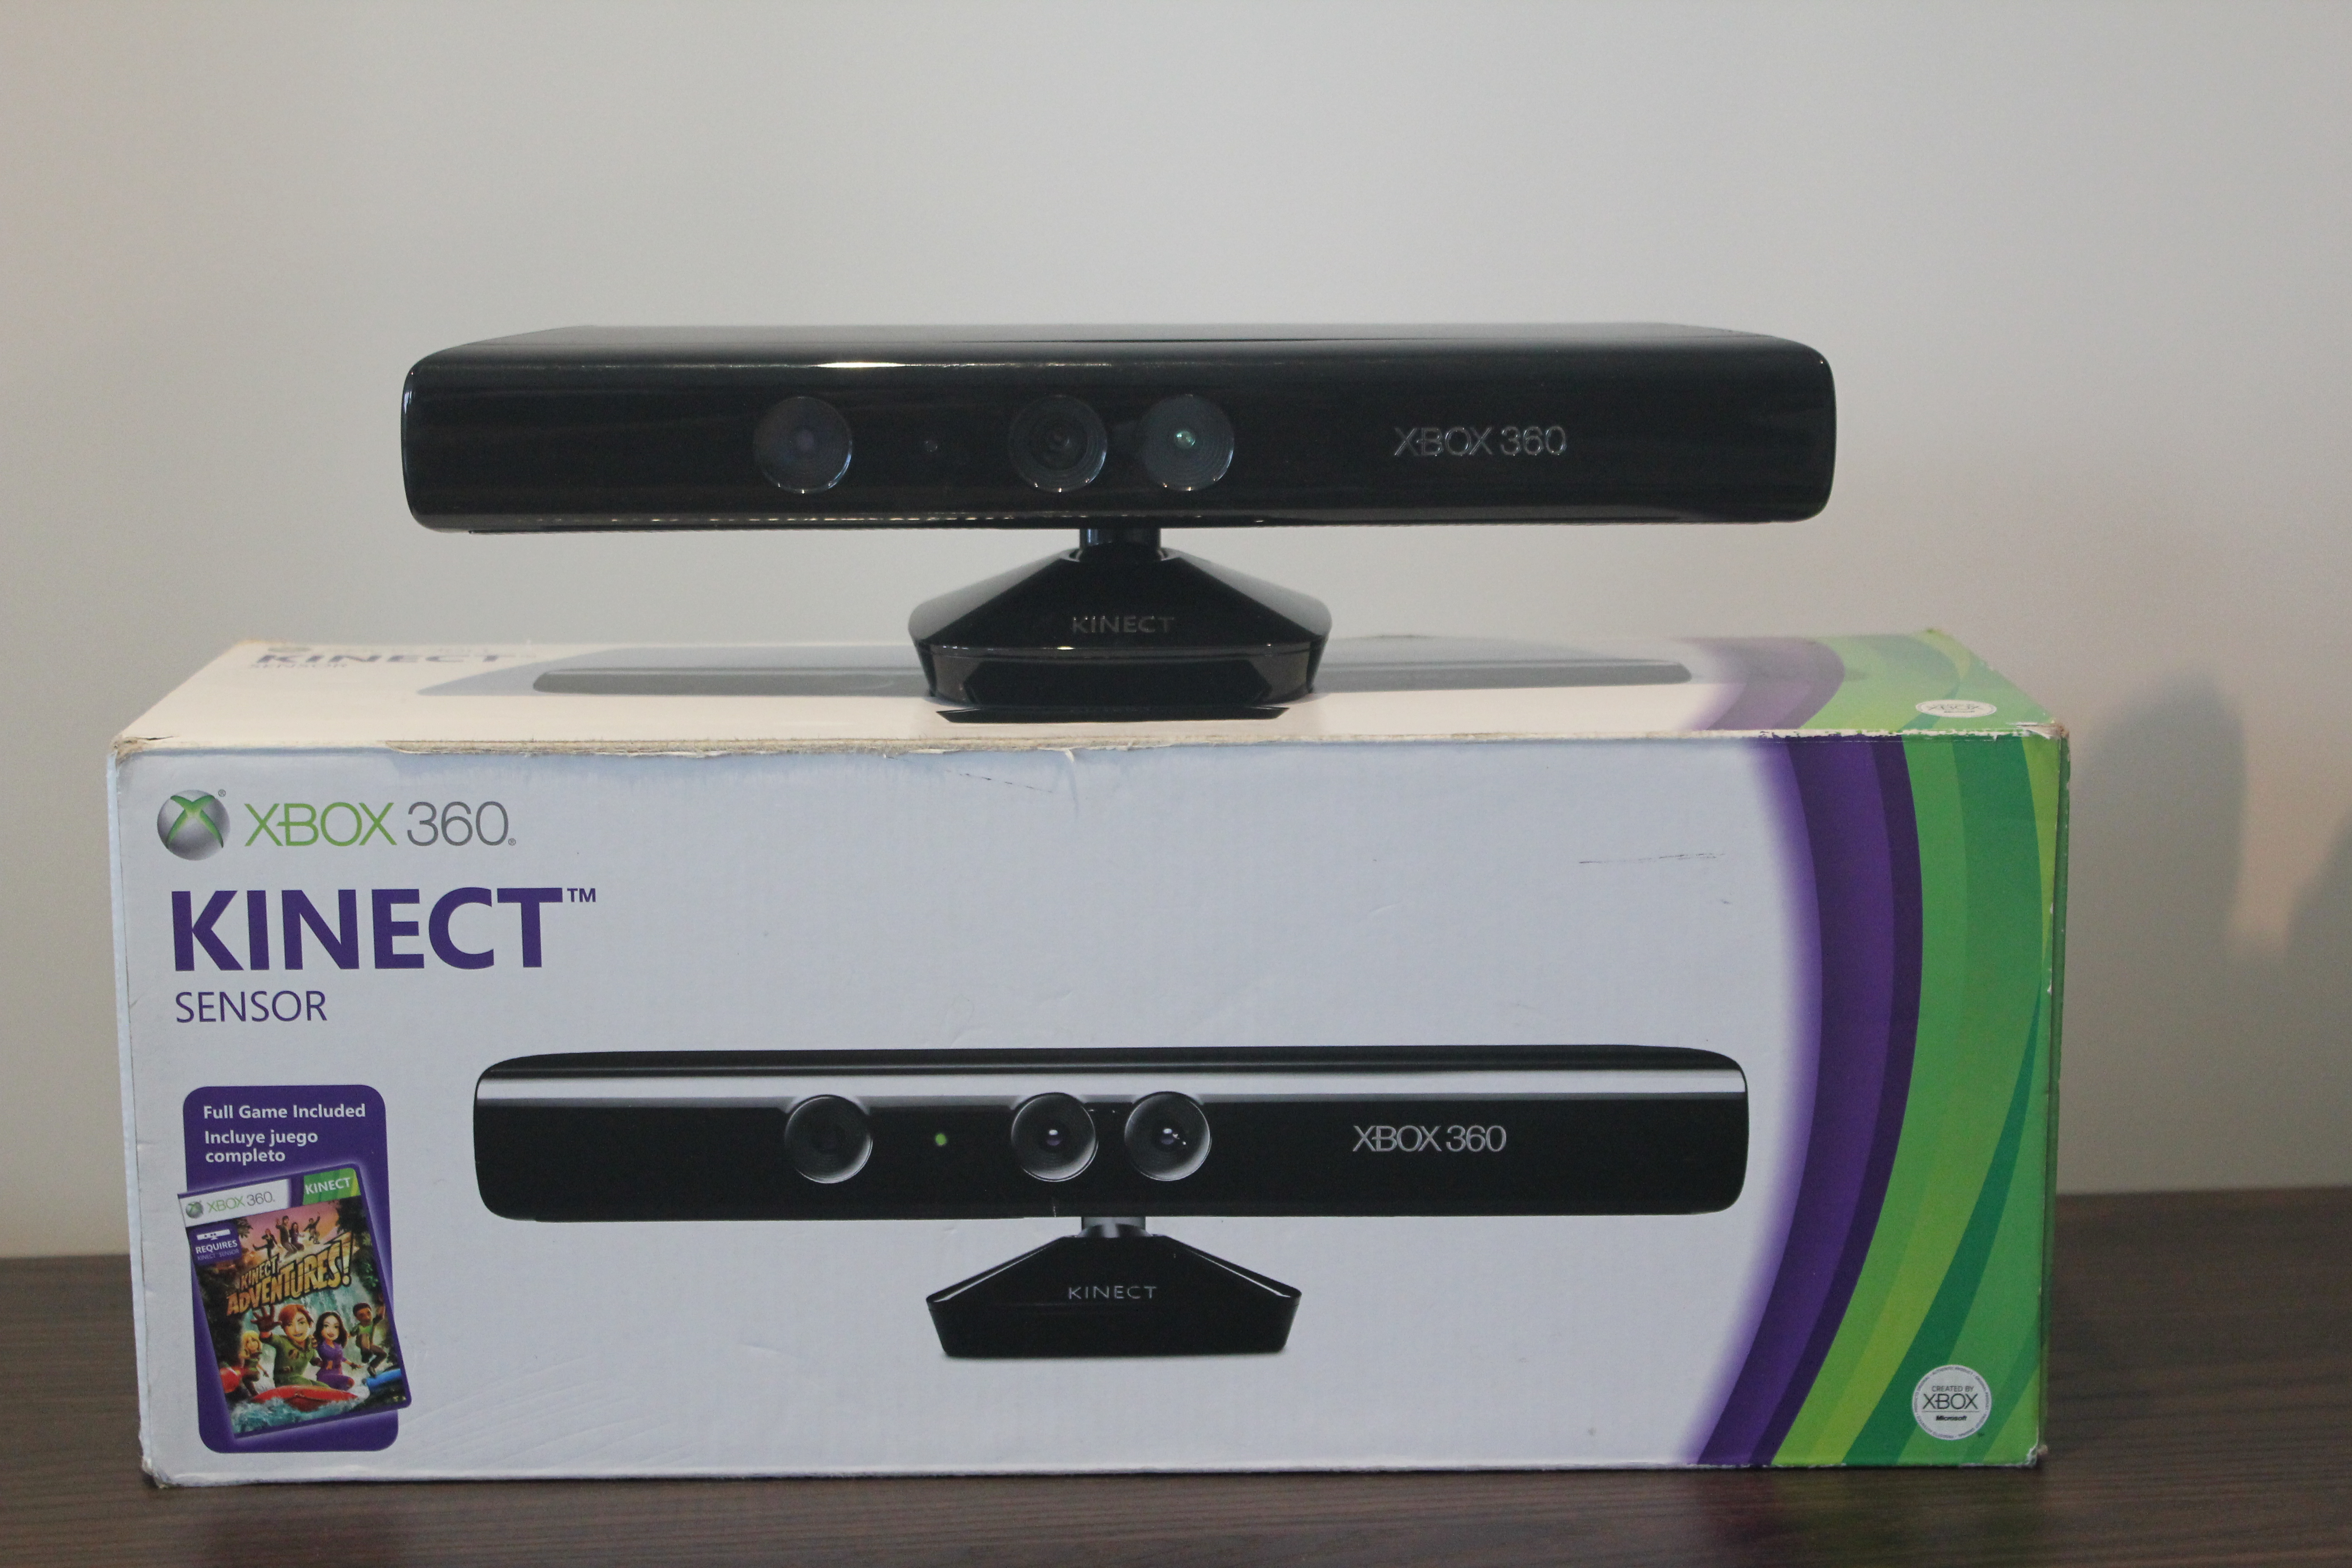
\includegraphics[scale=0.07]{figuras/Apendice/kinect.JPG}
		\end{center}
		\caption{Sensor Kinect da Microsoft.}
		\label{kinect}
	\end{figure}

	A Microsoft define o \textit{Kinect} como ``jogos sem necessidade de controle e experiência de entretenimento''. Porém, seu uso e inovação não se limita apenas no campo dos jogos eletrônicos (15).

	O \textit{Kinect} possui as seguintes especificações técnicas:

	\begin{itemize}
		\item Sensor
			\begin{itemize}
				\item Lentes com detecção de cores e profundidade
				\item Microfone de voz
				\item Motor de inclinação para ajuste do sensor
			\end{itemize}
		\item Campo de visão
			\begin{itemize}
				\item Campo de visão horizontal: 57 graus
				\item Campo de visão vertical: 43 graus
				\item Alcance físico da inclinação: (+/-) 27 graus
				\item Um alcance máximo de aproximadamente $\displaystyle 4.5$ metros para câmera de profundidade. 
			\end{itemize}
		\item Fluxo de Dados
			\begin{itemize}
				\item 320x240 16-bit depth a 30FPS
				\item 640x480 32-bit color a 30FPS
				\item 16-bit áudio a 16 kHz
			\end{itemize}
	\end{itemize}

Seu hardware é composto por câmeras que obtém imagens de cor, som e que utiliza iluminação infravermelha (IR) para obter dados de profundidade~\cite{kinect}. A Figura \ref{kinect_interno} apresenta a organização interna do \textit{Kinect} em alto nível.

	\begin{figure}[hbt]
		\begin{center}
			\includegraphics[scale=0.8]{figuras/2.FundamentacaoTeorica/kinect_interno.png}
		\end{center}
		\caption{Organização interna do Kinect~\cite{kinect}.}
		\label{kinect_interno}
	\end{figure}

Um chip especializado é responsável pelo processamento dos dados fornecidos pela câmera de profundidade correlacionando-os com as imagens de cor. O software interno ao \textit{Kinect} combina cada pixel com sua profundidade, processa os dados e os envia a máquina por meio de uma interface USB na forma de mapas de profundidades e imagens de cor~\cite{kinect}.


\chapter{Processamento da imagem}
\label{apend:processamento}

As etapas de processamento da imagem utilizadas nesse trabalho consistem na conversão em escala de cinza, corte, redimensionamento e equalização da mesma. Neste apêndice são mostrado trechos de códigos que implementam tais etapas utilizando a biblioteca \textit{OpenCV}.

\section{Escala de Cinza}

		\begin{lstlisting}[caption=Conversão de uma imagem para escala de cinza., label=list:grey-scale]
		IplImage* imageToGreyscale(const IplImage *imageSrc) {
			IplImage *imageGrey;

			// cria uma nova imagem do mesmo tamanho que a imagem passada como parametro e de 1 canal.
			imageGrey = cvCreateImage(cvGetSize(imageSrc), IPL_DEPTH_8U, 1);

			//converte o espaco de cor de imageSrc para o espaco de cor (cinza) da imageGrey
			cvCvtColor(imageSrc, imageGrey, CV_BGR2GRAY);

			return imageGrey;
		}
		\end{lstlisting}

\section{Corte da Imagem}

	\begin{lstlisting}[caption=Corte de uma imagem., label=list:crop]
		IplImage* crop(const IplImage *img, const CvRect region) {
			IplImage *imageTmp;
			IplImage *imageRGB;
			CvSize size;
			size.height = img->height;
			size.width = img->width;

			if (img->depth != IPL_DEPTH_8U) {
				printf("ERROR: img->depth de %d desconhecido ao inves de 8 bits por pixel passado a crop().\n", img->depth);
				exit(1);
			}

			// cria uma nova imagem (colorida ou em cinza) e copia os conteudos da imagem nela.
			imageTmp = cvCreateImage(size, IPL_DEPTH_8U, img->nChannels);
			cvCopy(img, imageTmp, NULL);

			// cria uma nova imagem da regiao detectada
			// seta a região de interesse que é ao redor da face
			cvSetImageROI(imageTmp, region);

			//copia a imagem de interesse na nova iplImage (imageRGB) e a retorna
			size.width = region.width;
			size.height = region.height;
			imageRGB = cvCreateImage(size, IPL_DEPTH_8U, img->nChannels);
			cvCopy(imageTmp, imageRGB, NULL);//copia somente a regiao

			cvReleaseImage(&imageTmp);
			return imageRGB;
		}
	\end{lstlisting}

\section{Redimensionamento}

	\begin{lstlisting}[caption=Redimensionamento de uma imagem., label=list:resize]
		IplImage* resize(const IplImage *origImg, int newWidth, int newHeight) {
			IplImage *outImg = 0;
			int origWidth, origHeight;

			if (origImg) {
				origWidth = origImg->width;
				origHeight = origImg->height;
			}

			if (newWidth <= 0 || newHeight <= 0 || origImg == 0 || origWidth <= 0 || origHeight <= 0) {
				printf("ERROR: Tamanho %dx%d desejado para imagem invalido\n.", newWidth, newHeight);
				exit(1);
			}

			// modifica as dimensoes da imagem, mesmo se a proporcao mude
			outImg = cvCreateImage(cvSize(newWidth, newHeight), origImg->depth, origImg->nChannels);
			cvResetImageROI((IplImage*) origImg);
			if (newWidth > origImg->width && newHeight > origImg->height) { // aumentar a imagem
				//CV_INTER_LINEAR muito boa para aumentar a imagem
				cvResize(origImg, outImg, CV_INTER_LINEAR); 

			} else { //diminuir a imagem
				//CV_INTER_AREA muito boa para diminuir a imagem, porem pessima para aumenta-la
				cvResize(origImg, outImg, CV_INTER_AREA);
			}

			return outImg;
		}
	\end{lstlisting}

\section{Equalização}

	\begin{lstlisting}[caption=Equalização de uma imagem., label=list:equalizacao]
		//cria uma imagem limpa na escala de cinza
		equalizedImg = cvCreateImage(cvGetSize(sizedImg), 8, 1); 

		// metodo que realiza "equalização de histograma"
		// normalizando o brilho e aumentando o contraste
		cvEqualizeHist(sizedImg, equalizedImg);
	\end{lstlisting}	










\chapter{JNI}
\label{apend:jni}

JNI (\textit{Java Native Interface}) é uma \textit{framework} que permite que
aplicações em Java possam chamar e serem chamadas por aplicações nativas e
bibliotecas escritas em outras linguagem tal como C, C++ e Assembly.
O propósito dessa abordagem é oferecer a possibilidade de que programadores
possam implementar funcionalidades não disponibilizadas pela API padrão do Java
ou até mesmo melhorar as já implementadas seja por questão de desempenho,
segurança ou outros.

Para implementar os metodos nativos basta criar uma função com a estrutura
\ref{list:estruturaJNI}. Quando a JVM executar o metodo ela invocará a função
definida e passará os parametros conforme o esperado \cite{jniDoc}. 

	\begin{lstlisting}[caption=HelloWorld.java., label=list:estruturaJNI]	
		JNIEXPORT void JNICALL Java_ClassName_MethodName(JNIEnv *env, jobject obj) {
			/*Implement Native Method Here*/
		}
	\end{lstlisting}
	
\section{HelloWorld}

	Para criar o primeiro programa utilizando a JNI basta criar os arquivos
	\ref{list:helloWorldJava}, \ref{list:helloWorldH},
	\ref{list:helloWorldC} e \ref{list:make} e no console executar \cite{jniDoc}:
	
	\textit{chmod +x make.sh}
	
	\textit{./make.sh}


	\begin{lstlisting}[caption=HelloWorld.java., label=list:helloWorldJava]
	class HelloWorld {
			static {
				System.loadLibrary("HelloWorld");
	    }
	    
	    private native void print();
	        
	    public static void main(String[] args) {
	    	new HelloWorld().print();
	    }   
	}
	\end{lstlisting}
	
	\begin{lstlisting}[caption=HelloWorld.h., label=list:helloWorldH]
	
		/* DO NOT EDIT THIS FILE - it is machine generated */
		#include <jni.h>
		/* Header for class HelloWorld */
		 
		#ifndef _Included_HelloWorld
		#define _Included_HelloWorld
		#ifdef __cplusplus
		extern "C" {
		#endif
		/*
		 * Class:     HelloWorld
		 * Method:    print
		 * Signature: ()V
		 */
		JNIEXPORT void JNICALL Java_HelloWorld_print(JNIEnv *, jobject);
		 
		#ifdef __cplusplus
		}
		#endif
		#endif
	\end{lstlisting}
		
	\begin{lstlisting}[caption=HelloWorld.c., label=list:helloWorldC]
		#include "jni.h"
		#include <stdio.h>
		#include "HelloWorld.h"
		 
		JNIEXPORT void JNICALL Java_HelloWorld_print(JNIEnv *env, jobject obj) {
		    printf("Hello World!\n");
		    return;
		}
	\end{lstlisting}
	
	\begin{lstlisting}[caption=make.sh., label=list:make]
		#!/bin/sh
		export LD_LIBRARY_PATH=$LD_LIBRARY_PATH:.
		javah HelloWorld
		gcc -shared -Wl,-soname,HelloWorld -o libHelloWorld.so HelloWorld.c \
			-I/usr/lib/jvm/java-6-openjdk/include \
			-I/usr/lib/jvm/java-6-openjdk/include/linux
		javac HelloWorld.java
		java HelloWorld
	\end{lstlisting}



\end{document}


